%%%%%%%%%%%%%%%%%%%%%%%%%%%%%%%%%%%%%%%%%%%%%%%%%%%%%%%%%%%%%%%%%%%%%
% PREAMBLE
%%%%%%%%%%%%%%%%%%%%%%%%%%%%%%%%%%%%%%%%%%%%%%%%%%%%%%%%%%%%%%%%%%%%%
%
% The following two commands will generate a PDF that follows all the requirements for submission
% and peer review.  Uncomment these commands to generate this output (and comment out the two lines below.)
%
% DOUBLE SPACE VERSION FOR SUBMISSION TO THE AMS
\documentclass[12pt]{article}
\usepackage{ametsoc}
\usepackage{subfigure}

\newcommand{\degree}{^\circ}
%
% The following two commands will generate a single space, double column paper that closely
% matches an AMS journal page.  Uncomment these commands to generate this output (and comment
% out the two lines above. FOR AUTHOR USE ONLY. PAPERS SUBMITTED IN THIS FORMAT WILL BE RETURNED
% TO THE AUTHOR for submission with the correct formatting.
%
% TWO COLUMN JOURNAL PAGE LAYOUT FOR AUTHOR USE ONLY
%%%%\documentclass[10pt]{article}
%%%%\usepackage{ametsoc2col}
%
%%%%%%%%%%%%%%%%%%%%%%%%%%%%%%%%%%%%%%%%%%%%%%%%%%%%%%%%%%%%%%%%%%%%%
% ABSTRACT
%
% Enter your Abstract here
%%%%%%%%%%%%%%%%%%%%%%%%%%%%%%%%%%%%%%%%%%%%%%%%%%%%%%%%%%%%%%%%%%%%%
\newcommand{\myabstract}{A new operational wave forecasting system has been implemented at the National Center for Environmental Prediction using the third release of WAVEWATCH III\texttrademark. The new system uses a mosaic of grids with two way nesting to simulate wave processes at global and regional scales in a single model. This global system replaces the older operational wave modeling suites $-$ NWW3, AKW, ENP and WNA. The new forecast system consists of eight grids at different resolutions to provide Weather Forecast Offices (WFOs) of the National Weather Service (NWS) and the different centers of NCEP with gridded model guidance of suitable resolution for all areas where they have the responsibility to provide gridded forecast products. New features in WAVEWATCH III, such as two way nesting between grids and carving out selected areas of the computational domain, allow us to increase the spatial resolution and global domain while at the same time optimizing the computational cost. Output from the model includes both point and field data. Field output data is now packed in GRIB2 format and apart from the standard mean wave parameters it also includes parameters of partitioned wave spectra. The partitioning is currently limited to three fields: wind-wave component, primary and secondary swells. The modeling system has been validated against data using a 5 year hindcast database.}
%
\begin{document}
%
%%%%%%%%%%%%%%%%%%%%%%%%%%%%%%%%%%%%%%%%%%%%%%%%%%%%%%%%%%%%%%%%%%%%%
% TITLE
%
% Enter your TITLE here
%%%%%%%%%%%%%%%%%%%%%%%%%%%%%%%%%%%%%%%%%%%%%%%%%%%%%%%%%%%%%%%%%%%%%
\title{\textbf{\large{A Multi-grid Wave Forecasting model: A new paradigm in operational wave forecasting}}}
%
% Author names, with corresponding author information. 
% [Update and move the \thanks{...} block as appropriate.]
%
\author{\textsc{Arun Chawla}
				\thanks{\textit{Corresponding author address:} 
				Arun Chawla, SAIC/MMAB/NCEP/EMC/NOAA, 
				5200 Auth Road Camp Springs MD. 
				\newline{E-mail: arun.chawla@noaa.gov}}
\and 
\centerline{\textsc{Hendrik L. Tolman, Vera Gerald}}\\% Add additional authors, different insitution
\centerline{\textit{\footnotesize{MMAB/EMC/NCEP/NOAA MD USA}}}
\and
\centerline{\textsc{Degui Cao, Todd Spindler}}\\
\centerline{\textit{\footnotesize{SAIC/MMAB/EMC/NCEP/NOAA MD USA}}}
\and
\centerline{\textsc{Jeffrey L. Hanson}}\\
\centerline{\textit{\footnotesize{USACE Field Research Facility, Duck NC}}}
\and
\centerline{\textsc{Eve-Marie Devaliere}}\\
\centerline{\textit{\footnotesize{UNC/USACE Field Research Facility, Duck NC}}
}}
%
% Formatting done here...Authors should skip over this.  See above for abstract.
\ifthenelse{\boolean{dc}}
{
\twocolumn[
\begin{@twocolumnfalse}
\amstitle

% Start Abstract (Enter your Abstract above.  Do not enter any text here)
\begin{center}
\begin{minipage}{13.0cm}
\begin{abstract}
	\myabstract
	\newline
	\begin{center}
		\rule{38mm}{0.2mm}
	\end{center}
\end{abstract}
\end{minipage}
\end{center}
\end{@twocolumnfalse}
]
}
{
\amstitle
\begin{abstract}
\myabstract
\end{abstract}
}
%%%%%%%%%%%%%%%%%%%%%%%%%%%%%%%%%%%%%%%%%%%%%%%%%%%%%%%%%%%%%%%%%%%%%
% MAIN BODY OF PAPER
%%%%%%%%%%%%%%%%%%%%%%%%%%%%%%%%%%%%%%%%%%%%%%%%%%%%%%%%%%%%%%%%%%%%%
\section{Introduction}
NCEP provides guidance for wind waves and ocean swells using the third
generation spectral wave model WAVEWATCH III\texttrademark
\cite[]{tolman-02}. The model uses a third order propagation scheme
that minimizes numerical diffusion and a parallel code was developed
to increase computational speed \cite[]{tolman-02d}. Until recently
the operationla forecast system consisted of a suite of wave models
that included a global forecast model (NWW3 $-$
\citealt{tolmanetal-02}) and three regional models for the Alaskan
Waters (AKW $-$ \citealt{chao-akw}), Eastern North Pacific (ENP $-$
\citealt{chao-enp}) and Western North Atlantic (WNA $-$
\citealt{chao-wna}). Boundary conditions for the regional models were
obtained from the global model. Computational costs limited the global
operational model to a grid of $1.25\degree \times 1\degree$, and the
regional models to a $0.25\degree \times 0.25\degree$ grid. While this
resolution is adequate for providing guidance to regional forecasts,
coastal forecasts (put out by the various Weather Forecast Offices)
are needed at grids with resolutions of 5km or higher. Furthermore,
boundary conditions for the regional grids are obtained from the
global model, but the higher resolution effects are not passed back
from the regional grids to the global grid.

The WAVEWATCH III computational model has moved away from a paradigm
of representing the computational domain with a single grid to one
where the domain is represented as a mosaic of multiple grids in which
there is two way exchange of information (from low resolution to high
resolution grids and vice versa) between overlapping grids
\cite[]{tolman-08}. Using multiple grids within the same model allows
for locally increasing resolution (inlets etc.) but at the same time
localizing the effects of the CFL limits on temporal resolution and
thus minimizng the computational cost.

The multi-grid version of WAVEWATCH III has been used to develop a new
operational forecast system for NCEP. The modeling system (herafter
referred to as NMWW3) has been operational since December 2007 and has
replaced the older modeling suites (NWW3, AKW, WNA and ENP).


\section{WAVEWATCH III Upgrades}

Many significant changes have been introduced in the multi-grid
version of WAVEWATCH III (version 3 and higher) and a more detailed
description of these changes can be found in \cite{tolman-08}. Broadly
these changes fall into 3 categories and a brief overview of these
changes are provided here.
 
\subsection{Mosaic approach to wave modeling}
\label{sec:MGW}

Instead of representing the computational domain by a single grid as
was done in the past, the new version of WAVEWATCH III now allows the
domain to be represented by an arbitrary number of grids of different
resolution. Grids are ranked according to their resolution, with the
lower resolution grids having a lower rank, and grids with similar
resolution having the same rank. Each grid acts as a separate wave
model, however there is full two-way interaction between the grids in
the regions where they overlap. Data for the boundary points of the
higher ranked grids are obtained from the lower ranked grids that
these points lie in. Similarly in the lower ranked grids, points that
lie inside the domain of higher ranked grids receive spatially
averaged data from the latter. This allows sea states that develop in
high resolution areas to propagate out to lower resolution
areas. Overlapping grids with the same rank are reconciled in their
area of overlap. This mosaic approach to wave modeling allows us to
use a single model driver to generate forecasts at several different
resolutions over the computational domain, thus, greatly simplifying
operational requirements. Also higher resolution grids can be limited
to coastal regions (where their impact is the greatest), while the
open ocean can be respresented with a coarser grid thus saving on the
computational cost associated with the CFL limitations on time steps.

The boundary points (where data is passed from the lower to higher
ranked grids) can now be defined at the edge of the grid, precluding
the need for spurious land values along the edge as was the practice
in WAVEWATCH III v 2.22 \cite[]{tolman-02}. The new model also allows
boundary points to be defined inside the grid, making a distinction
between land, active and excluded points. This feature has been
heavily used in developing an optimal forecast model as it allows us
to follow the coast line and carve out regions within the same grid
where higher resoultion computations are desired (section~\ref{sec:NMWW3}).

\subsection{Partitioning of wave spectra}
\label{sec:PRT}

Apart from providing guidance on the overall wave height operational
wave forecast models also try to provide guidance on swell and wind
wave fields to mariners. Traditionally this has been done by using a
frequency cutoff in the spectrum to separate wind and swell
fields. Such a cutoff can partition energy into a swell field even if
there are no peaks in the energy spectrum. A new algorithm developed
by \cite{hanson-04,hansonetal-09} to partition the energy spectrum has
been added to the model. It is based on a digital image processing
watershed algorithm \cite[]{vincent-91} and divides the energy
spectrum into partitions based on the number of peaks in the
spectrum. Figure~\ref{fig:imeds_part} provides an example of how the
partitioning algorithm works. Each partition represents a sea state
and bulk spectral parameters (significant wave height, peak period and
direction) across the partition as well as the number of partitions
are now part of model output.

\subsection{New Physics}

Two new source terms have been added to the model to better simulate
physical processes. One is the linear growth parametrization of
\cite{cavaleri-81} together with a filter for low frequency energy
\cite[]{tolman-92}. This term has been added to consistently spin up
the model from quiescent conditions and to better simulate the initial
wave growth. The second source term is a depth induced breaking term
from \cite{battjes-78} that simulates energy dissipation due to surf
zone breaking. This term has been added to extend the applicability of
the model into shallow water environments which has become
increasingly possible with the development of the mosaic approach to
wave modeling. The source term is based on the criterion that all wave
heights exceeding a maximum height in the surf zone will break and the
energy dissipation rate is based on dissipation of a turbulent bore. A
parallel approach to improve the overall physics packages in WAVEWATCH
III is also in progress and will be reported elsewhere.

\section{Multi - grid forecast model (NMWW3)}
\label{sec:NMWW3}

A single operational multi-grid forecast model (hereby referred to as
NMWW3) was designed to replace the existing suite of global and
regional operational models. The new forecast model was designed to
run on the same schedule as the old models, i.e. 4 forecast cycles a
day (at 0Z, 06Z, 12Z and 18Z). Each cycle consists of a 189 hour long
run with 9 hours of hindcast and 180 hours of forecast. Restart files
are generated at the 6 hour time step to be used as starting
conditions for the next cycle.

\subsection{Grids}

The main aim of developing the NMWW3 model was to provide guidance
forecasts for the WFOs (Weather Forecast Offices) and the regional
prediction centers (Ocean Prediction Center and Tropical Prediction
Center) at a suitable resolution within the available
computational constraints. The WFOs provide forecasts for the US
coastal waters on grids with a 5km or finer resolution. These grids
extend out to approximately 60 nautical miles along the US west coast
and 40 nautical miles along the US east coast. The regional forecasts
on the other hand are provided on $10'$ resolution grids by the two
prediction centers. The regions that fall under the mandate of
regional forecasts include the US west and east coasts, Alaska,
Hawaii, Gulf of Mexico and some of the islands in the South Pacific.

To provide appropriate guidance forecasts, the global domain was
divided into eight grids $-$ one global $1/2\degree$ grid, four
regional grids ($1/6\degree$ grids for the US East Coast including the
Gulf of Mexico and the Caribbean Sea, for the US West Coast and for
the Pacific Ocean including Hawaii and select islands in the Eastern
Pacific, and a $1/4\degree \times 1/6\degree$ grid for Alaska), and
three coastal grids ($1/15\degree$ grids for the US East Coast
including the coastal waters of Puerto Rico and for the US West Coast
including the coastal waters of Hawaii, and an $2/15\degree \times
1/15\degree$ grid for Alaska). Figure~\ref{fig:grids} shows the map
representation of the different grids. In contrast the older models
had a grid resolutions of $1.25\degree \times 1\degree$ for the global
model and $1/4\degree$ for the regional models. The global domain
excludes the polar ice cap regions and extends from -77.5$\degree S$
to 77.5$\degree N$ and 180$\degree W$ to 180$\degree E$. Separation of
the computational domain into eight different grids was done to
optimize the parallel implementation within the constraints of desired
regional grid resolutions. Note that the lower resolution grids extend
to the coast, creating a full overlap with higher resolution grids.

Optimal high resolution regional grids were designed by taking
advantage of the model's flexibility in assigning boundary points
inside a grid (section~\ref{sec:MGW}). This is highlighted by the mask
generated for the Pacific Ocean $1/6\degree$ grid
(Fig.~\ref{fig:wnp_mask}). This grid covers Hawaii and other smaller
islands in the Pacific Ocean where higher resolution results are
desired. In the new model, points where high resolution results are
not needed can be excluded. This significantly reduces the number of
active points (where model computations are carried out) and the
subsequent computational cost. The flexibility to assign individual
points as land, active, inactive or boundary allows us to design
efficient coastline following high resolution grids as seen in
Fig.~\ref{fig:grids}. 

Figure.~\ref{fig:Hs_grids} shows a snapshot of wave heights at the
three different resolutions individually as well as the composite wave
heights for the 120 hour forecast for the 12Z cycle on Oct 26$^{\rm
th}$, 2007. The composite image was generated by plotting results for
all grids consecutively (ordered from low to high resolution) and
shows the seamless distribution of wave heights across the
grids. Comparing the global grid image with the composite picture, we
can see the impact of the high resolution grids in the better
representation of the Hawaiian and Aleutian island chains. This example
showcases the robustness of the two-way communication (between grids)
algorithm. More examples of this can be seen in \cite{tolman-08}.

The impact of the high resolution coastal grids can be clearly seen in
simulations of land falling hurricanes such as Katrina
(Fig.~\ref{fig:kat}). The coast line is better represented in NMWW3
and the addition of shallow water wave breaking physics leads to more
realistic estimates of wave heights with respect to water depth
(Fig.~\ref{fig:kat_ratio}). It should be noted that the aim of these
simulations is to highlight the differences in the WNA and NMWW3
models and as such do not account for the underlying surge that would
have a major impact on the wave field of a land falling
hurricane. Coupling of surge models with wave models in operations is
part of our future implementation plans.

\subsection{Obstruction model}

The algorithm for using obstruction grids to simulate blocking effects
from unresolved islands \cite[]{tolman-03} has been an integral part
of WAVEWATCH III since 2002 and remains unchanged in the new
version. However, these grids were developed manually and in a
multi-grid model where there can be multiple grids such an approach
can be a fairly tedious and onerous task. Furthermore, due to the two
way coupling of the grids, the obstruction grids need to be consistent
across grids in the regions of overlap. In a manual approach where the
choices are subjective this is not guaranteed. To alleviate these
concerns a grid generation package was developed
\cite[]{chawla-07,chawla-08} for WAVEWATCH III to automate the grid
generation process and create consistent grids across different
resolutions. In this package obstruction grids are generated using the
GSHHS shoreline database. The GSHHS database \cite[]{wessel-96}
contains an exhaustive global list of shoreline boundaries (over
180000) and covers land bodies ranging from small atolls to large
continents. This package has been used to develop the bathymetric and
obstruction grids for the multi-grid model and its impact can be seen
in the case of hurricane Katrina (Fig.~\ref{fig:kat}) where the
blocking effects of the Chandaleur islands is not accounted for in the
WNA model in-lue of these islands not being represented in the
obstruction grids but are accounted for in NMWW3 since these islands
are represented in the GSHHS database (and therefore the obstruction
grids for NMWW3).

\subsection{Forcings} 

The wave model is forced by the 10 meter winds, air-sea temperature
difference and ice data. In the new multi-grid model the individual
grids can obtain the external forcings from either a single grid that
covers the entire domain (data is interpolated or averaged from the
forcing grid to the computational grid internally in the code) or have
unique forcing data sets for each grid. The former approach is used in
NMWW3 as it precludes the need to develop individual forcing files for
each grid as well as maximizes consistency of winds across the
different grids. Sea ice concentration data are updated once a day
over a global $1/12\degree$ grid using an automated passive microwave
analysis \cite[]{grumbine-96}. Forecast winds are obtained from the
Global Forecast System (GFS $-$ previously known as AVN/MRF)
\cite[]{kanamitsu-89,kanamitsuetal-91,caplanetal-97}. Hindcast winds
are obtained from the Global Data Assimilation System (GDAS)
\cite[]{kanamitsu-89,derberetal-91} and uses global observations to
provide initial conditions for the GFS model. GDAS provides the best
estimate of the winds and is the primary reason why we run 9 hours of
hindcast simulation. Apart from the hindcast winds GDAS is also used
to determine the initial sea surface temperature. All the wind data
are provided on a 3h time step. Wind data are obtained from the lowest
sigma level of the atmospheric model on a $1/2\degree$ spatial grid
and converted to 10m winds assuming a nuetrally stable vertical
boundary layer.

Since the interpolation of wind fields is done internally for each
grid (and is not a part of the pre-processing) NMWW3 was designed so
that it can run side by side with GFS model. A time stamp file is used
to determine the available wind data and to control the forward
propagation of the model. When new wind data becomes available this
file is updated and the model allowed to propagate forward in
time. This way, the model run is now completed within a few minutes of
the GFS 180h wind file being made available, significantly improving
the delivery time of forecast products. This approach has been
feasible in NMWW3 due to the highly modular code design of WAVEWATCH
III consistent with the Earth System Modeling Framework (ESMF)
concepts.
 
\subsection{Outputs}

There are two types of output data in NMWW3 $-$ field data and point
data. This is similar to the output fields of the older wave
models. However, there are some distinct differences.

Field data consist of the mean characteristics of the ocean spectral
data represented on a spatial domain. The same field outputs that were
part of the old operational models are also available in the new
model. However the new model also includes a partitioning algorithm
that separates a 2d spectrum into individual sea states
(section~\ref{sec:PART}). The sea states are separated into wind seas
and swells, with the bulk characteristics of each sea state being part
of the output.

The wind wave portion of the spectrum is given by a single component,
even if the spectrum in this region has multiple peaks. For the partitioned
output the wind wave fraction is given by
\begin{equation}
W = E^{-1}E|_{Up > c}
\end{equation}
where $E$ is the total energy, $E|_{Up > c}$ is the portion of the
energy spectrum directly under the influence of the winds and
corresponds to part of the spectrum where the projected wind speed
$U_p$ is greater than the phase speed $c=\sigma/k$. The projected wind
speed is given by
\begin{equation}
U_p = C_m U_{10}\cos(\theta-\theta_w)
\end{equation}
where $U_{10}$ is the 10 meter wind, $\theta$ and $\theta_w$ are the
directions of the waves and wind respectively, and $C_m$ is a constant
multiplier that allows for moving the wind-swell boundaries to lower
frequencies.

The partitioning algorithm does not put a limit on the number of
possible swell fields in the spectrum. However, in the operational
model output we currently limit ourselves to the first two swell
fields (based on local wave height partition) which are referred to as
the primary and secondary swells.

Field data is packed using the GRIB2 standard from World
Meteorological Organization (WMO) which provides greater flexibility
in meta data handling and more efficient packing options than the
earlier GRIB standard (which is used in the older modeling suites). To
allow for future increases in the number of output swell fields, swell
parameters are stored as vertical levels, with the first level
corresponding to the primary swell.

Like the older forecast model suites, point output data in NMWW3
provides both detailed spectral data as well as the mean spectral
characteristics. As of now the mean spectral characteristics for the
point outputs are not obtained using the partitioning algorithm but
that is expected to change in the near future. Since in NMWW3 a point
location can be in multiple grids, the data are retrieved from the
highest rank grid (highest resolution) that the point lies in. As
before, the list of points include current and old buoy locations,
virtual buoy locations as well as boundary locations (for
collaboration projects within and outside NOAA using NMWW3 results as
boundary conditions for external models). This list has been
expanded to include buoy points from NDBC (National Data Buoy Center),
ENCAN (Environment Canada), GOMOOS (Gulf of Maine OOS), IDT (Irish
Department of Transport), UKMO (UK Met Office), SHOM (Service
Hydrographique et Oceanographique de la Marine) and METFR (Meteo
France) among others.

\section{Validation}

The NMWW3 model has been in operations since December 2007. As part of
operations an archive of select model results (at collocated altimeter
and buoy locations) is maintained. Apart from that, a database of
hindcast runs extending from Feb 2005 to the present has also been
developed. This database uses the same settings as the NMWW3 model,
with the addition of a ninth grid in the arctic region to expand the
northern boundary from $77.5\degree$ N to $83\degree$ N\footnote{This
additional grid is going to be introduced into NMWW3 later this
year}. Both the forecasts and the hindcast datasets have been used to
obtain a baseline global skill assesment of the multi-grid model. The
study spans several years to look for seasonal trends.

\subsection{Altimeter Comparisons}

For altimeter comparisons we rely on the Jason-1 satellite data to
provide estimates of $H_s$. The altimeter data used is the so called
``fast delivery'' data which is available in near real time. Since the
modeling system went into operations daily files of altimeter and
collocated model (for hindcast and several forecast periods) are being
generated and archived as part of the operational suite of
products. Error metrics have been computed using month long records of
this daily archive to ensure global coverage. Calibration and
validation of the fast delivery satellite data with buoy measurements
was done by \cite{tolmanetal-06} and as part of this study were
confirmed again using the 2008 altimeter data set (figure not shown).

A de-spiking algorithm is used to remove spikes in the altimeter
data. The de-spiking algorithm also accounts for islands that lie
along the altimeter track, but are too small to be resolved in the
model domain. One of the issues with satellite data is that the data
sets are very noisy, which leads to erroneously larger estimates of
scatter indices, particularly in periods of low wave heights. To
separate the instrument noise from model-data deviations, a running
average is used to smooth the altimeter data.

Figure~\ref{fig:sih_global} shows the scatter index (SI) computed
using raw and averaged altimeter data as a function of the forecast
period. The SI for any particular month is computed using the
collocated model and data over the entire global domain for that
period. Model data at multiple synoptic times of the forecast are
collocated with the altimeter data to provide a global skill
assessment of NMWW3. The error metric does not show any seasonal
variability and this will also be seen in the buoy data later in the
paper. There is also a significant difference between the raw and the
averaged data but not too much difference between the three different
levels of averaging. One of the dangers of smoothing data along the
altimeter track is that we may mis-represent systems with sharp
fronts. We thus want the minimal averaging window that provides
accurate error metrics. The SI grows more slowly over the first 48
hours of forecast and faster after that. A scatter index estimate
alone is not a good measure of the skill of the forecast (as it does
not account for biases and large index estimates may be driven by very
small wave heights observations). That said, over the global domain,
indices in the range of mid 20's and below, provide valuable guidance
information to forecasters. With that in mind, NMWW3 provides
good forecasts out to 96 hours, and anything beyond that should be
viewed with a greater degree of uncertainty.

Moving from an overall SI measure to a spatial map of indices
(Fig.~\ref{fig:SI_map}) we see that in general the indices are lower
at the eastern end of a basin as opposed to the western end (true for
both the Pacific and Atlantic basin). This is because winds in general
move from west to east, so the western part of the basin is an area of
wave generation and dominated by wind waves, which is a more dynamic
and localized wave field. Thus even if the model gets the wave growth
right, but misses the location, there would be significant error. On
the other hand, the eastern end of the basin is more swell dominated,
which tend to be much more stable and spread out (in space) in
comparison to the wind waves, hence leading to better comparisons
between model and data.

The overall bias measure as a function of forecast hour
(Fig.~\ref{fig:bih_global}) shows the same increasing trend that was
observed in the Scatter Index plot, indicating that the GFS winds are
getting stronger as a function of forecast hour. On the other hand,
the bias maps (Fig.~\ref{fig:bias_map_js1}) show a seasonal
variability in the Northern Hemisphere that is not seen in the SI
plots. During the winter months we see a positive bias in the Pacific
basin that extends from the center of the basin all the way to the
western coastline of the continental United States. This feature is
also seen to a smaller degree in the Atlantic basin. At the same time
the western part of the basins show a persistent negative bias. The
nature of these biases will be studied in greater detail in the
analysis of buoy data later in this section.

The bias maps also show a persistent positive bias over large regions
in the Southern Hemisphere. These biases have increased considerably
in comparison to the older NWW3 model (see
Fig.~\ref{fig:bias_map_alt}). For the period corresponding to this
figure, the wave model still did not have the island obstruction
algorithm of \cite{tolman-03} implemented, thus leading to the
bulls-eye patterns behind major island chains in the bias
maps. Accounting for this, we still see a positive bias over large
swathes of the Southern Hemisphere in NMWW3 that was absent in
NWW3. Even though there have been considerable changes between the two
systems, the underlying physics have remained largely unchanged (with
the exception of shallw water wave breaking and a linear growth term
that comes into play in the initial stages of wind wave growth from
quiescent conditions). To confirm that the changes in the bias
patterns are not driven by changes to the modeling system, we also
plotted the biases for the same period as in
Fig.~\ref{fig:bias_map_js1} using NWW3
(Fig.~\ref{fig:bias_map_js1_nww3}). Since the bias patterns for 2008
are similar for the two modeling systems, and distinctly different
from the patterns in 2002, the changes are driven by something other
than changes to the modeling system. Even though we have used data
from two different satellites (ERS-2 and Jason-1) to highlight the
recent development of persistent bias in the Southern Hemisphere,
these patterns are also confirmed by the buoy comparisons in the next section.
 
A possible reason for persistent increased biases in the Southern
Hemisphere is that the representation of the winds in this region by
the GFS model has changed since the last time that the wave model was
tuned (2000-2001). Fig.~\ref{fig:wind_stats} shows the wind statistics
(from the GFS model) over water in both the Southern and Northern
Hemisphere. Since 2005, we can see a clear upward shift in the higher
wind speeds, leading to a significant change in the $99^{th}$
percentile curves, with minimal impact on the average wind speeds. And
since wave growth is a non-linear process, this manifests as a
positive bias in the wave model. The winds in the Northern Hemisphere
over the same period did not show any significant changes. It remains
to be seen if a new database of high resolution re-analysis winds
(currently under development at NCEP) will show the same results.
  
\subsection{Buoy Comparisons}

Comparisons of wave model results with in-situ buoy data are very
useful in developing temporal records of model performance. To
quantify seasonal and long term changes in model skill we have
compared buoy data with a 5 year hindcast database that has been
developed using similar settings as the forecast model. The winds used
in developing the archive are the GDAS analysis winds that are used in
the forecast model during the hindcast part of the simulation. The
buoy data comes from a central archive being maintained by the
European Center for Meteorological Weather Forecasting (ECMWF) as part
of a data exchange program. This program has been set up under the
auspices of the Joint Technical Comission for Oceanography and Marine
Meteorology (JCOMM) to facilitate inter-comparison of operatinoal wave
modeling capability and includes several operational centers
\cite[]{bidlotetal-07}. The data archive consists of bulk spectral
parameters from over 250 buoys all over the
world. The hourly buoy data have been averaged over a $\pm 2$ hr
interval centered at the 4 synoptic time cycles (0,6,12 and 18) at
which model forecasts are run. Processing and quality control of these
data are done at ECMWF. 

Fig.~\ref{fig:ecmwf_buoys} shows the locations of the different
buoys. The buoys have been grouped by region, and only those regions
for which the results are shown in this paper are identified by
color. The error metrics for the different regions as a function of
time can be seen in Fig.~\ref{fig:ecmwf_buoys_err}. The seasonal
biases that was alluded to in section~\ref{sc:anal}.\ref{sc:alt_comp}
can be clearly seen in the time series plots. The buoys along the US
East Coast and in the Alaskan waters show a negative bias while the
buoys along the US West Coast show a positive bias pattern. These are
very consistent with the bias maps in
Fig.~\ref{fig:bias_map_js1}. Just like in the eastern part of the
Pacific basin, a positive bias pattern is also seen in the eastern
part of the Atlantic basin (European buoys) though the magnitudes
(with the exception of one year) are generally weaker. We can also see
the development of the same persistent positive bias in the buoys of
the Southern Hemisphere. The data indicates that these patterns have
started to grow since 2006, and this growth corresponds very well with
the change in the energetic wind speeds of the GFS model in the
Southern Hemisphere (Fig.~\ref{fig:wind_stats}). SI measures do not
show much of the seasonal trend seen in the bias plots and tend to be
fairly low everywhere. Like the altimeter data, buoy data also shows
the tendency for the indices to be larger in buoys that lie in areas
dominated by wind seas (such as the US East Coast) as opposed to
swells (US West Coast).

\subsection{Spectral Comparisons}

\section{Conclusions}

\begin{acknowledgment} 
Start acknowledgments here.
\end{acknowledgment}

% Use appendix}[A], {appendix}[B], etc. etc. in place of appendix if you have multiple appendixes.
%\ifthenelse{\boolean{dc}}
%{}
%{\clearpage}
%\begin{appendix}
%\section*{\begin{center}Appendix Title Is Entered Here (Primary heading)\end{center}}
%\subsection{First appendix secondary heading}

%\subsection{Second appendix secondary heading}

%\subsubsection{First appendix tertiary heading}

%\subsubsection{Second appendix tertiary heading}

%\paragraph{First appendix quaternary heading}

%\paragraph{Second appendix quaternary heading}

%\end{appendix}

% Create a bibliography directory and place your .bib file there.
\ifthenelse{\boolean{dc}}
{}
{\clearpage}
\bibliographystyle{./ametsoc}
\bibliography{./bibliography/references}

%%%%%%%%%%%%%%%%%%%%%%%%%%%%%%%%%%%%%%%%%%%%%%%%%%%%%%%%%%%%%%%%%%%%%
% FIGURES
%%%%%%%%%%%%%%%%%%%%%%%%%%%%%%%%%%%%%%%%%%%%%%%%%%%%%%%%%%%%%%%%%%%%%

\begin{figure}[t]
\noindent\includegraphics[angle=0,width=19pc]{./figures/imeds_part.eps}
\caption{Wave partitioning of a 2D spectrum. White lines denote the partition boundaries. (0 $\rightarrow$ wind wave component; 1 $\rightarrow$ primary swell; 2 $\rightarrow$ secondary swell).}
\label{fig:imeds_part} 
\end{figure}

\begin{figure}[t]
\noindent\includegraphics[angle=-90,width=19pc]{./figures/mww3_res.eps}
\caption{Grids for NMWW3. Grid resolution given in minutes}
\label{fig:grids}
\end{figure}

\begin{figure}[t]
\subfigure[Original Mask]{\includegraphics[angle=-90,width=19pc]{./figures/pacific_10m_mask.eps}}
\hspace*{0.5in} \subfigure[Final Mask]{\includegraphics[angle=-90,width=19pc]{./figures/pacific_10m_mask2.eps}}
\caption{Original and final masks for the Pacific grid. Mask values of
0, 1, 2 and 3 correspond to land, active, boundary and inactive points
respectively. Active points are reduced significantly from the
original (147426) to the final (5873) mask.}
\label{fig:wnp_mask} 
\end{figure}

\begin{figure}[t]
\subfigure[Global Grid]{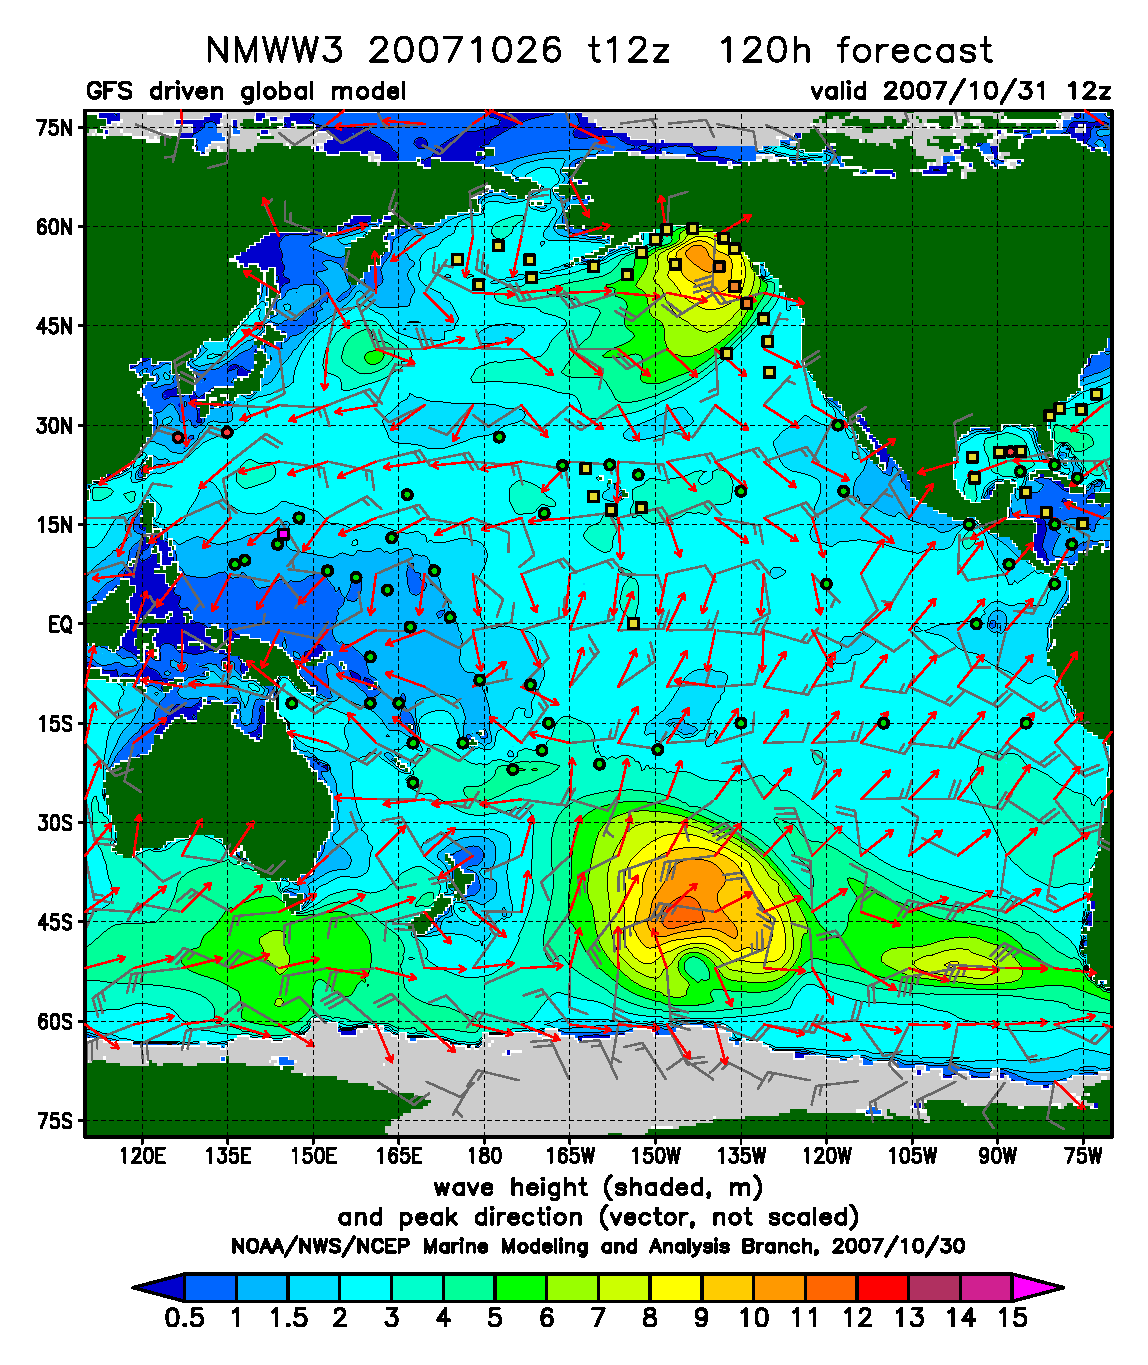
\includegraphics[angle=0,width=7cm]{./figures/pacific_global.eps}}\hspace*{0.5in}
\subfigure[Regional Grids]{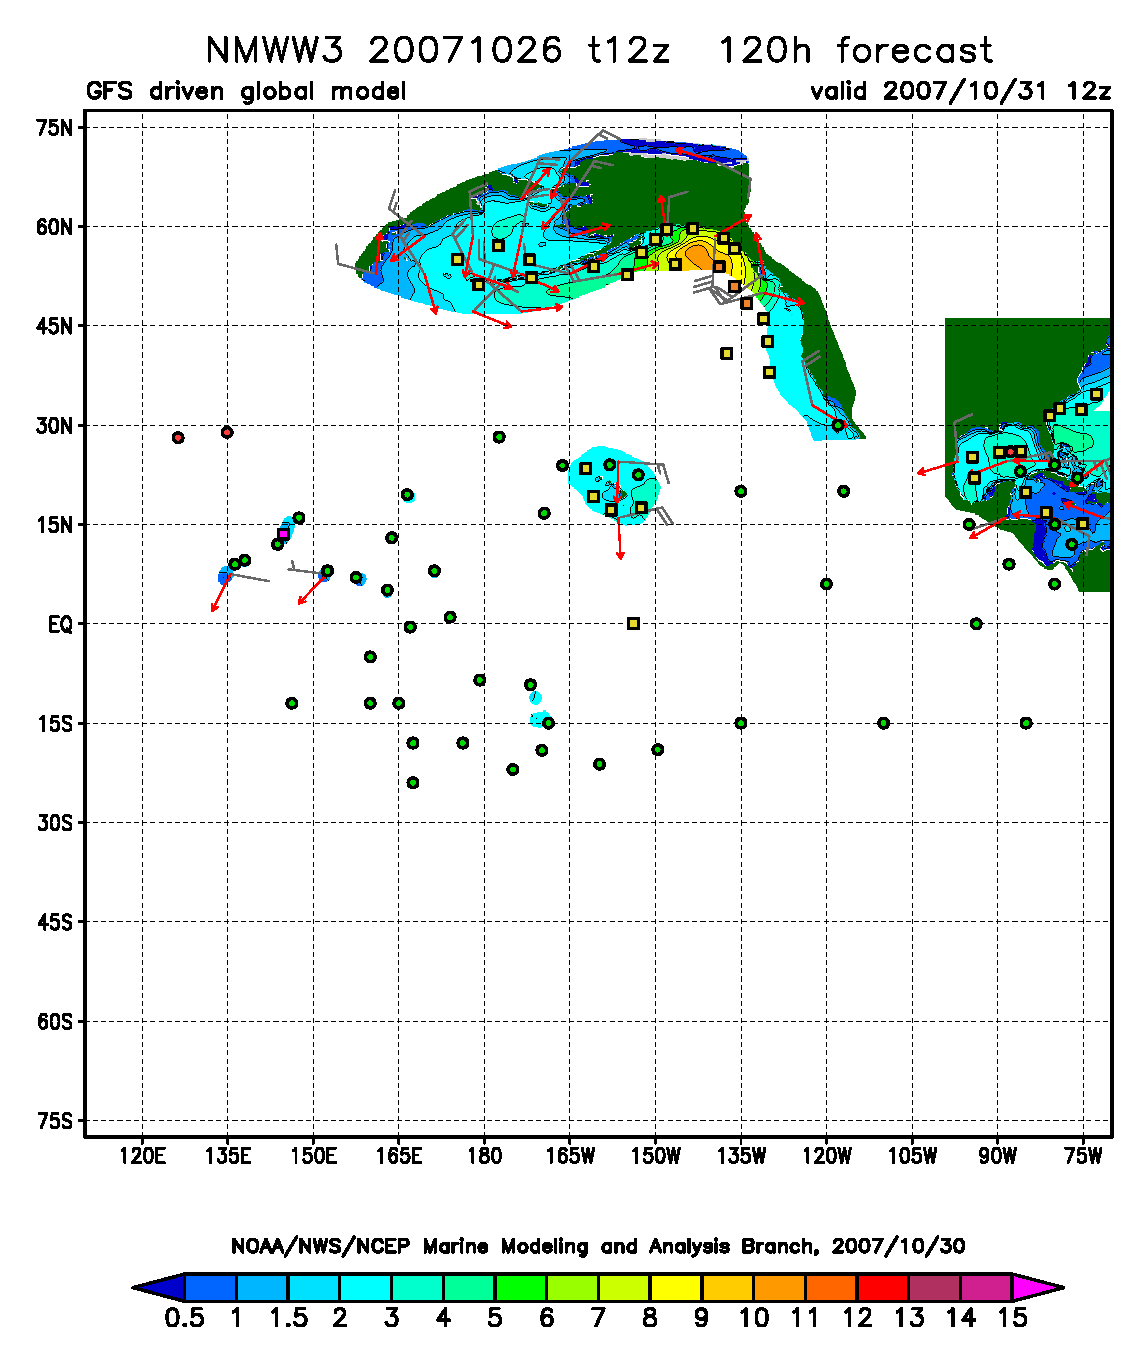
\includegraphics[angle=0,width=7cm]{./figures/pacific_regional.eps}}\\
\subfigure[Coastal Grids]{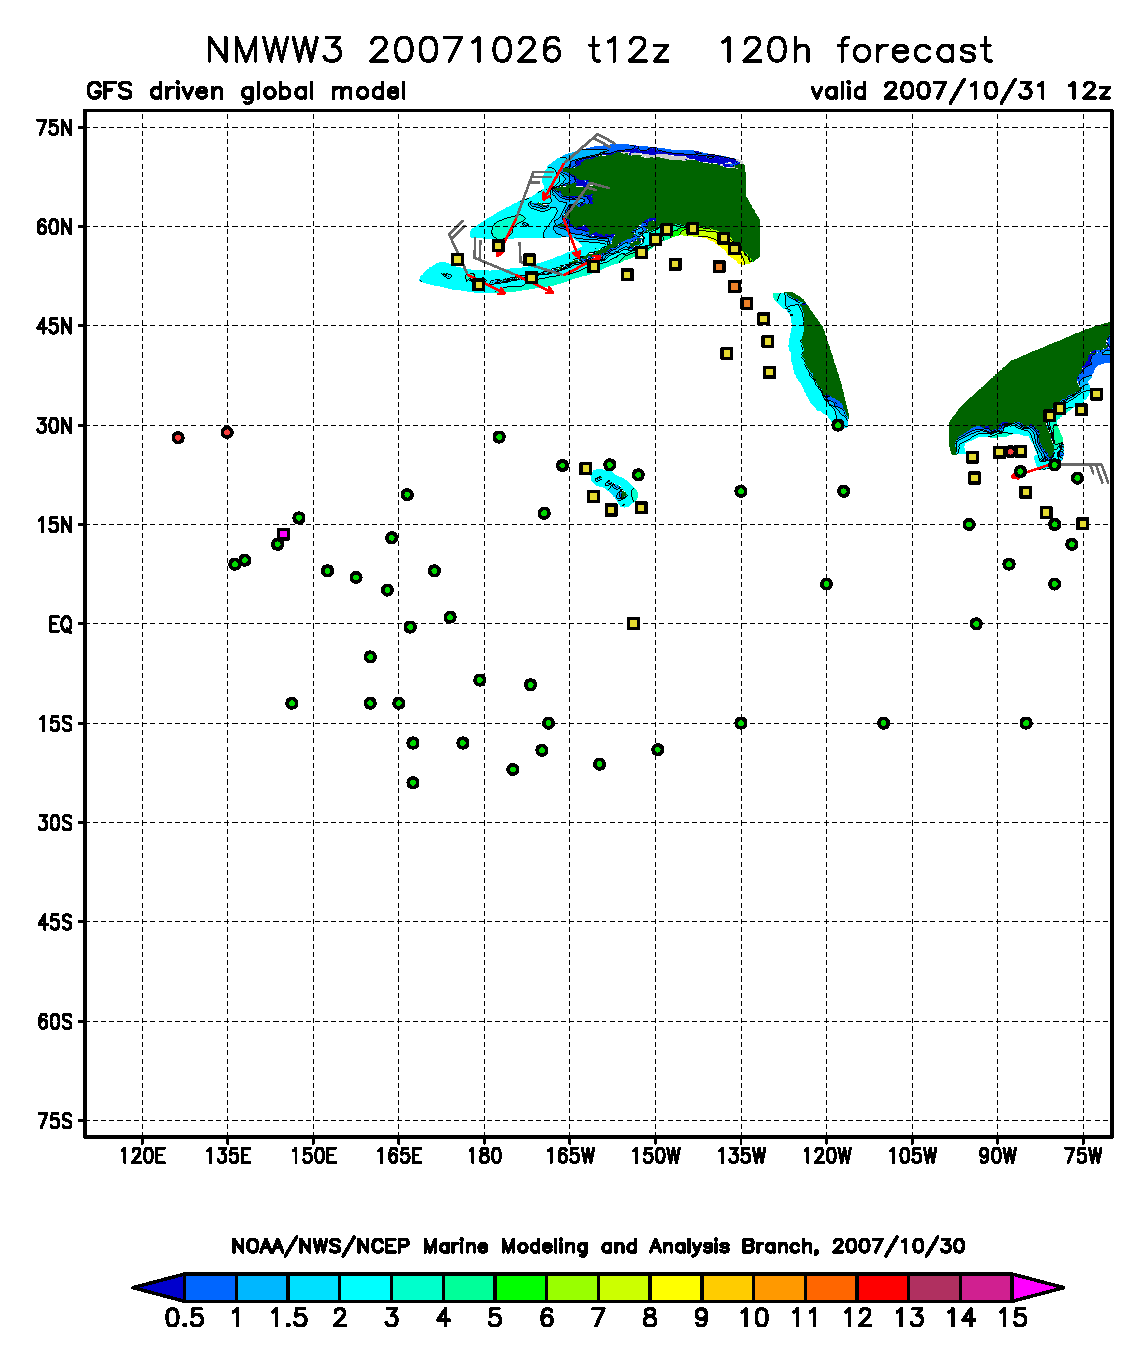
\includegraphics[angle=0,width=7cm]{./figures/pacific_coastal.eps}}
\hspace*{0.5in}
\subfigure[Composite]{\includegraphics[angle=0,width=7cm]{./figures/pacific_all.eps}}
\caption{Snapshot of wave height distribution at the different grid resolutions}
\label{fig:Hs_grids}
\end{figure}

\begin{figure}[t]
\subfigure[WNA model]{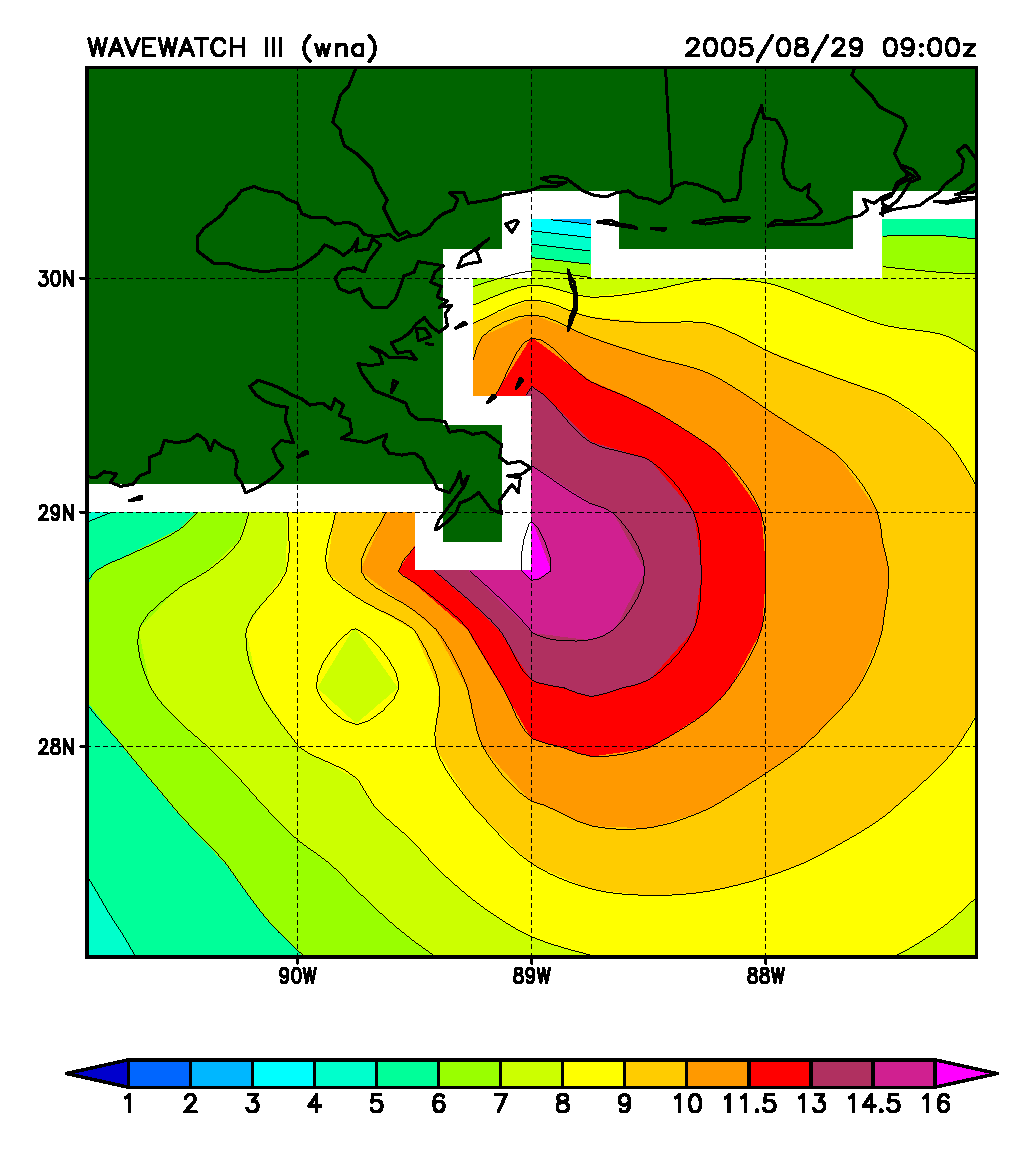
\includegraphics[angle=0,width=6.75cm]{./figures/Katrina_wna_hs.eps}}
\subfigure[NMWW3 model]{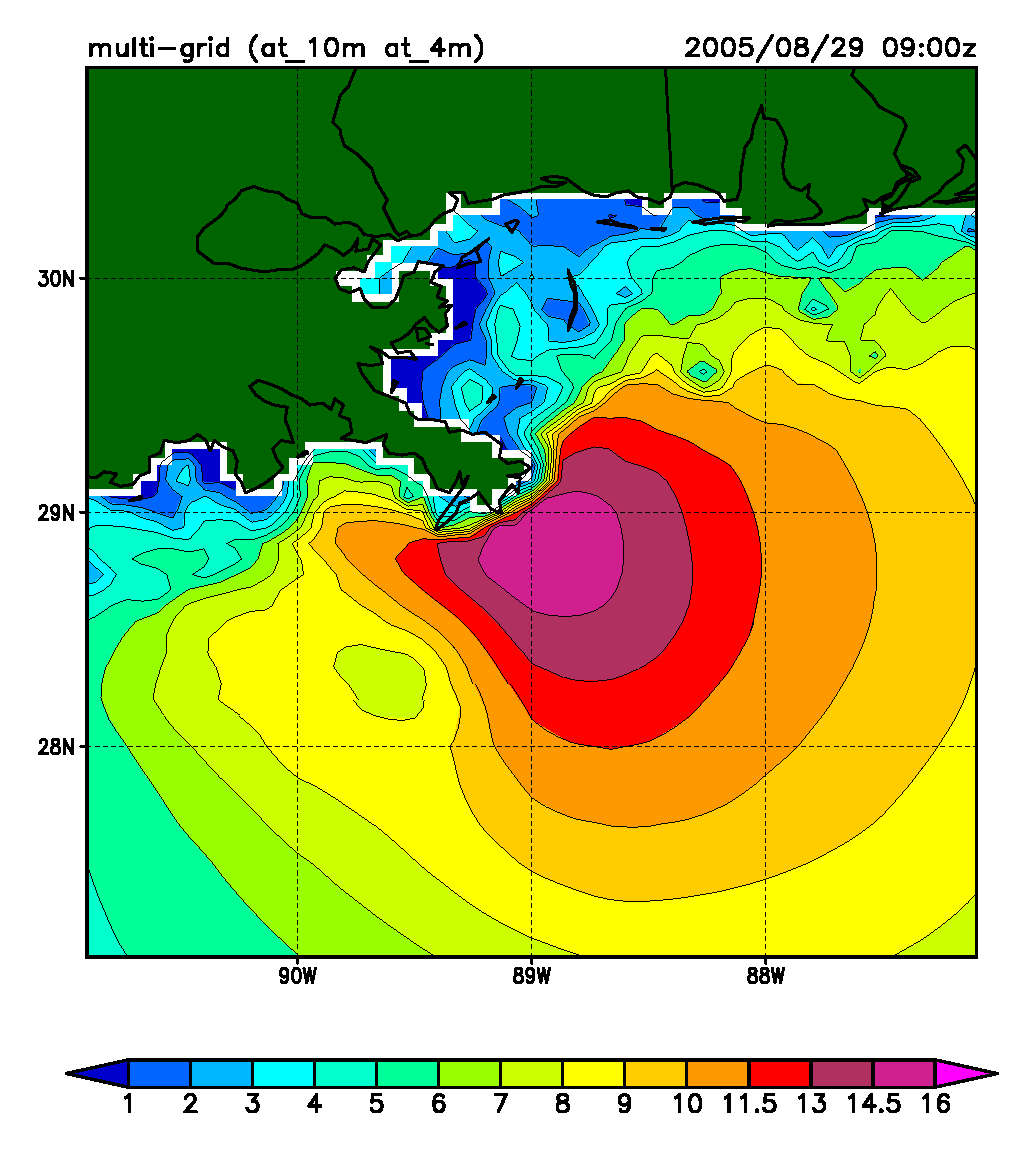
\includegraphics[angle=0,width=6.75cm]{./figures/Katrina_multiSdb_hs.eps}}
\caption{Significant wave heights at land fall during hurricane Katrina}
\label{fig:kat}
\end{figure}

\begin{figure}[t]
\subfigure[WNA model]{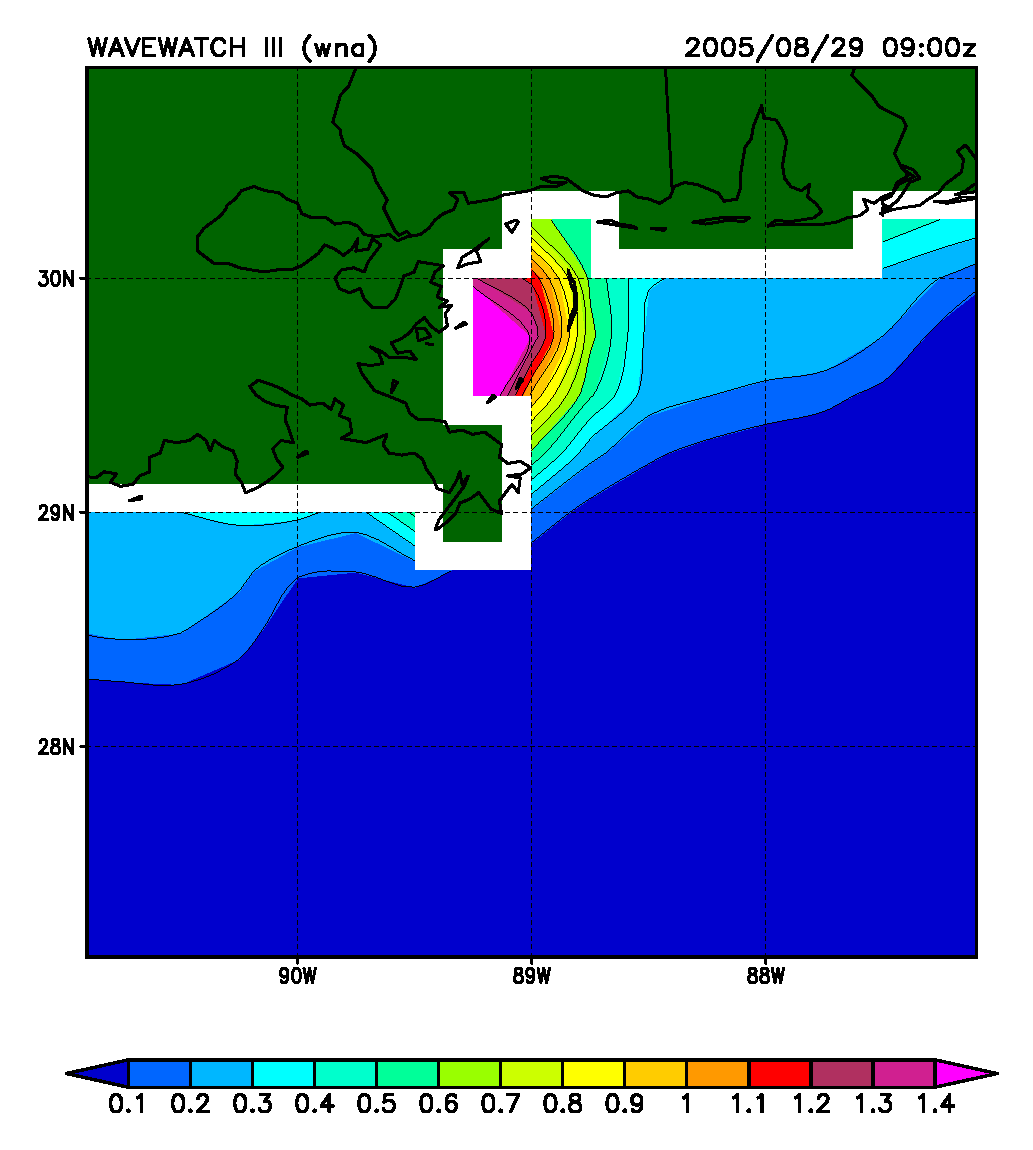
\includegraphics[angle=0,width=6.75cm]{./figures/Katrina_wna_ratio.eps}}
\subfigure[NMWW3 model]{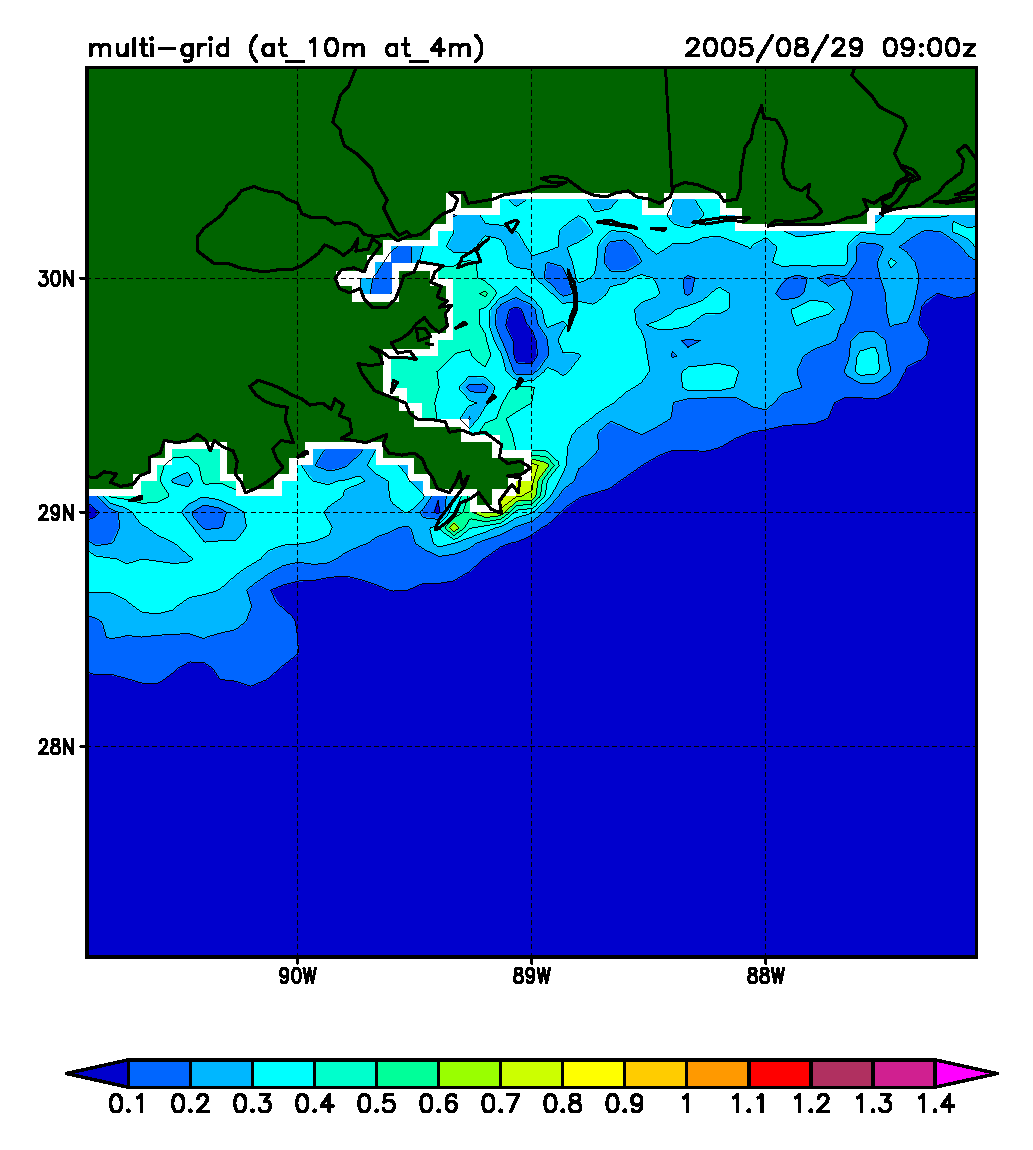
\includegraphics[angle=0,width=6.75cm]{./figures/Katrina_multiSdb_ratio.eps}}
\caption{Wave height to depth ratio at land fall during hurricane Katrina}
\label{fig:kat_ratio}
\end{figure}

\begin{figure}[t]
\subfigure[Overall Spectrum]{\includegraphics[angle=0,width=7cm]{./figures/pacific.hs.f120h.eps}}\hspace*{0.5in}
\subfigure[Wind wave component]{\includegraphics[angle=0,width=7cm]{./figures/pacific.hs_ws.f120h.eps}}\\
\subfigure[Primary swell]{\includegraphics[angle=0,width=7cm]{./figures/pacific.hs_sw1.f120h.eps}}
\hspace*{0.5in}
\subfigure[Secondary swell]{\includegraphics[angle=0,width=7cm]{./figures/pacific.hs_sw2.f120h.eps}}
\caption{Snapshot of wave height distribution for individual components}
\label{fig:Hs_part}
\end{figure}

\begin{figure}[t]
\subfigure[Overall Spectrum]{\includegraphics[angle=0,width=7cm]{./figures/pacific.tp.f120h.eps}}\hspace*{0.5in}
\subfigure[Wind wave component]{\includegraphics[angle=0,width=7cm]{./figures/pacific.tp_ws.f120h.eps}}\\
\subfigure[Primary swell]{\includegraphics[angle=0,width=7cm]{./figures/pacific.tp_sw1.f120h.eps}}
\hspace*{0.5in}
\subfigure[Secondary swell]{\includegraphics[angle=0,width=7cm]{./figures/pacific.tp_sw2.f120h.eps}}
\caption{Snapshot of peak period distribution for individual components}
\label{fig:tp_part}
\end{figure}

\begin{figure}[t]
\noindent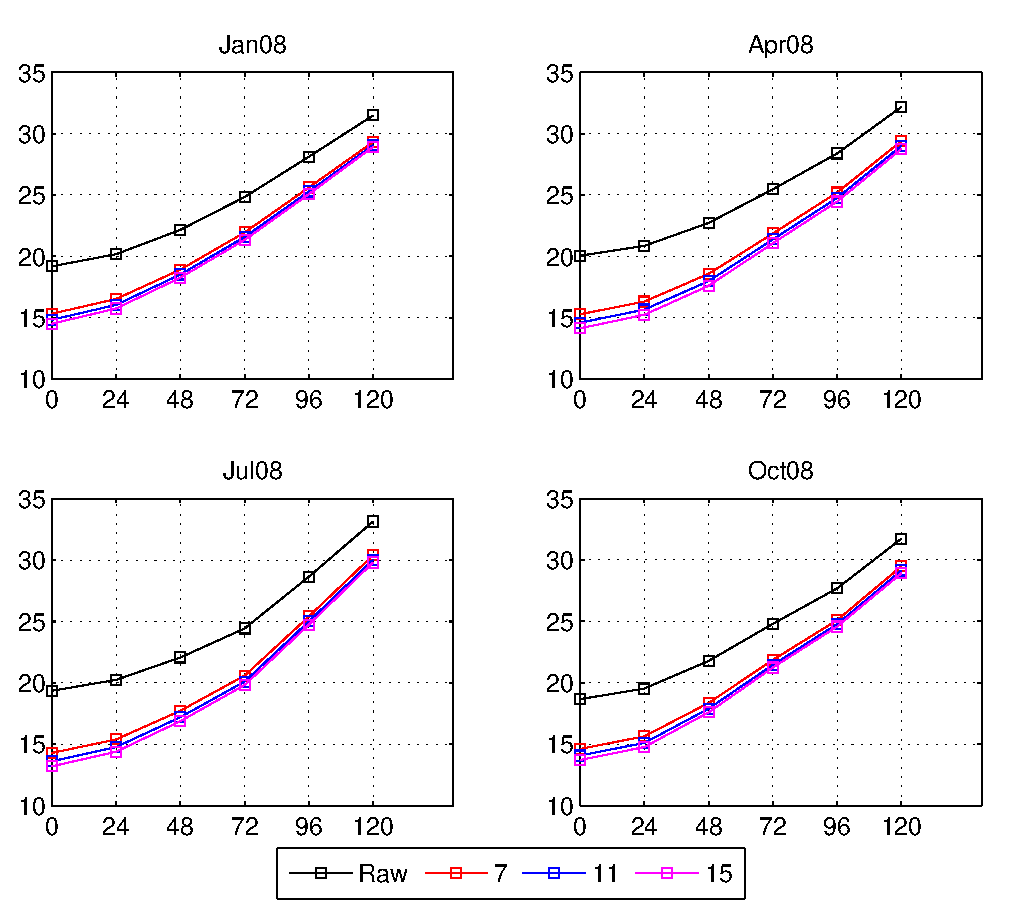
\includegraphics[width=19pc]{./figures/glo_30m_sih_comp.eps}
\caption{Scatter Index of $H_s$ as a function of forecast hour for four different months. Different lines correspond to different levels of smoothing}
\label{fig:sih_global}
\end{figure}

\setcounter{subfigure}{0}
\begin{figure}[t] 
\subfigure[Hindcast]{\includegraphics[width=7.5 cm]{./figures/SIHmap2_js1_global_HIND_200801_avg15.eps}}
\hspace*{0.25in}
\subfigure[48 Hr Forecast]{\includegraphics[width=7.5 cm]{./figures/SIHmap2_js1_global_F048H_200801_avg15.eps}} \\
\subfigure[72 Hr Forecast]{\includegraphics[width=7.5 cm]{./figures/SIHmap2_js1_global_F072H_200801_avg15.eps}}
\hspace*{0.25in}
\subfigure[96 Hr Forecast]{\includegraphics[width=7.5 cm]{./figures/SIHmap2_js1_global_F096H_200801_avg15.eps}}
\caption{Scatter Index map of $Hs$ for different periods of the forecast cycle. Map is generated by binning collocated model and altimeter data into 2$\degree$ $\times$ 2$\degree$ bins. Collocated data from January through March 2008 is used to provide enough points per bin for statistical analysis. A 3-point running average along the longitudes and latitudes is also applied to remove the signature of the tracks}
\label{fig:SI_map}
\end{figure}

\begin{figure}[t]
\noindent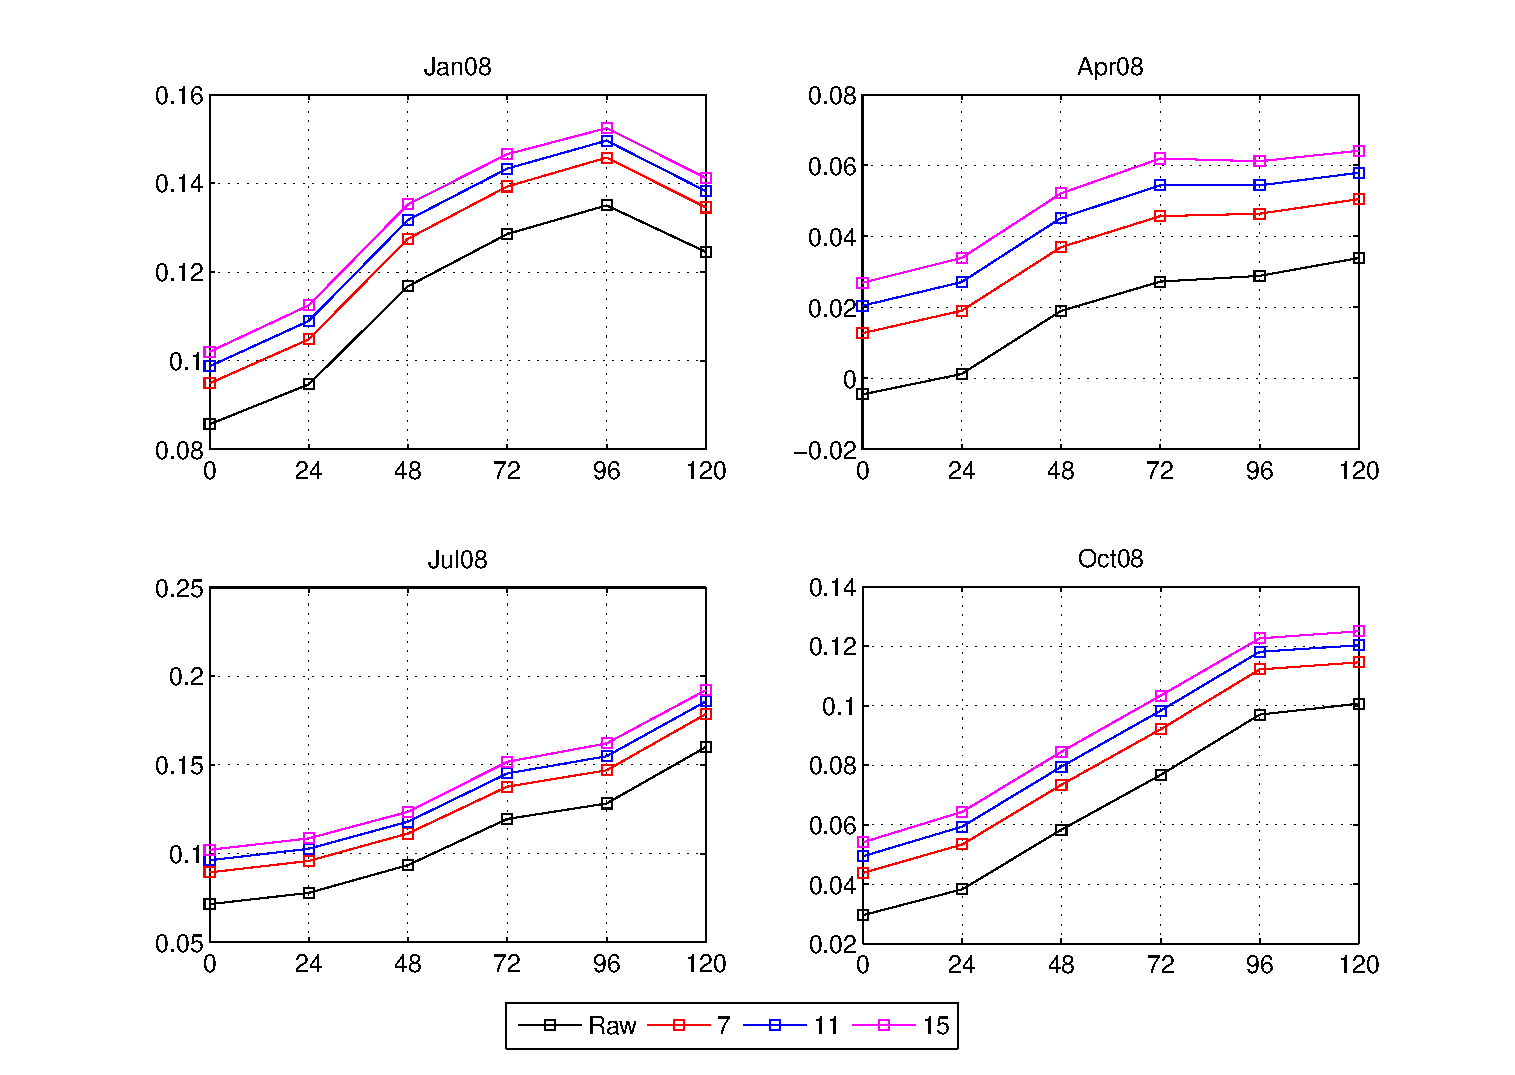
\includegraphics[width=19pc]{./figures/glo_30m_bih_comp.eps}
\caption{Bias (model - data) in $H_s$ (in m) as a function of forecast hour for four different months. Different lines correspond to different levels of smoothing}
\label{fig:bih_global}
\end{figure}

\setcounter{subfigure}{0}
\begin{figure}[t] 
\subfigure[Jan $-$ Mar]{\includegraphics[width=7.5 cm]{./figures/biasmap2_js1_global_HIND_200801_avg15.eps}}
\hspace*{0.25in}
\subfigure[Jul $-$ Sep]{\includegraphics[width=7.5 cm]{./figures/biasmap2_js1_global_HIND_200807_avg15.eps}}
\caption{Bias maps of $Hs$ hindcast simulations during the winter (a) and summer (b) periods. Bias maps are generated the same way as the SI maps (see caption of Fig~\ref{fig:SI_map} for details)}  
\label{fig:bias_map_js1}
\end{figure}

\begin{figure}
\noindent\includegraphics[width=19pc]{./figures/biasmap2_alt_global_HIND_200201_avg15.eps}
\caption{Bias map of wave hindcasts for the period Jan - Mar 2002, using the NWW3 model. Satellite data is from ERS-2.} 
\label{fig:bias_map_alt}
\end{figure}

\begin{figure}
\noindent\includegraphics[width=19pc]{./figures/biasmap2_js1_nww3_HIND_200801_avg15.eps}
\caption{Bias map of wave hindcasts for the period Jan - Mar 2008, using the NWW3 model. Satellite data is from Jason-1.} 
\label{fig:bias_map_js1_nww3}
\end{figure}

\setcounter{subfigure}{0}
\begin{figure}[t]
\subfigure[Southern Hemisphere]{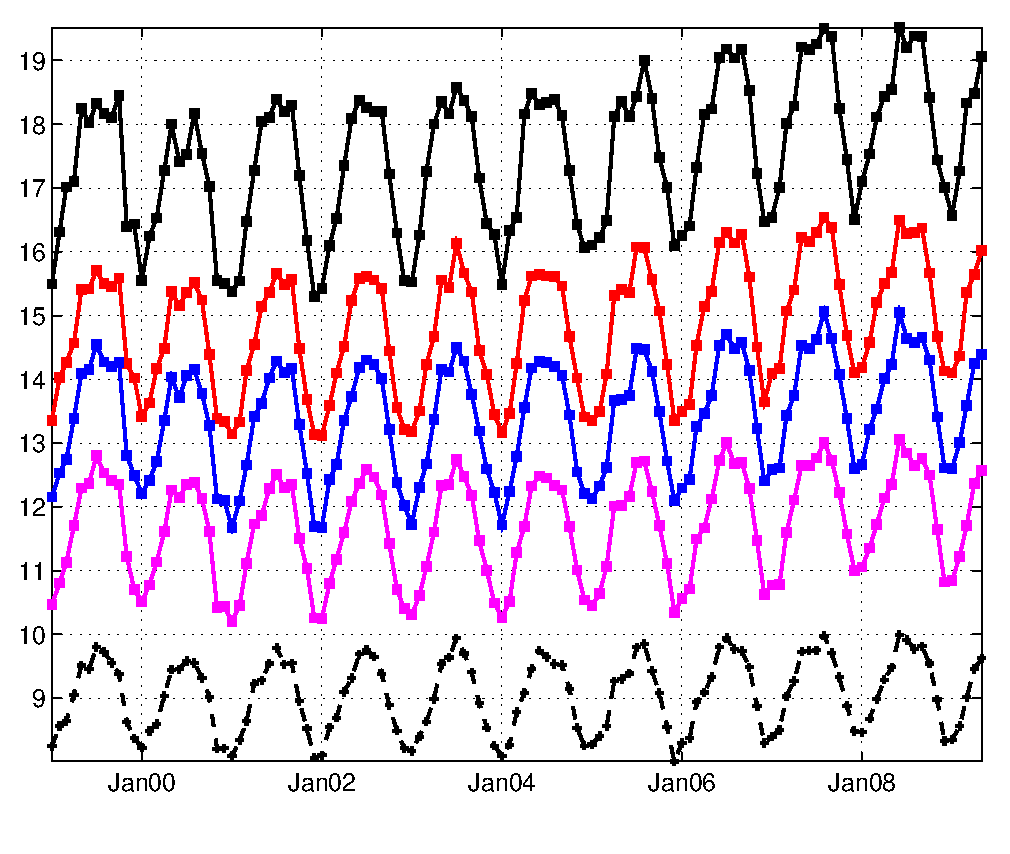
\includegraphics[width=7.5cm]{./figures/wave_clim_south.eps}}
\hspace*{0.25in}
\subfigure[Northern Hemisphere]{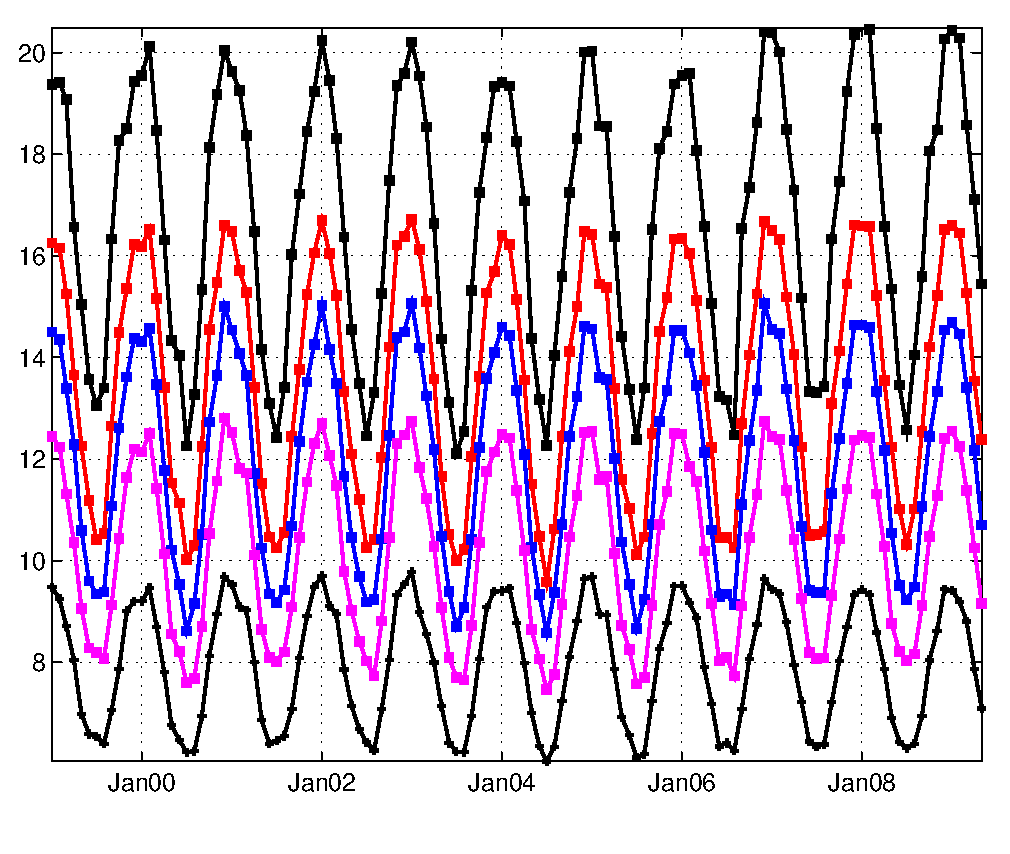
\includegraphics[width=7.5cm]{./figures/wave_clim_north.eps}}
\caption{Wind speed statistics for the 10m winds from the GFS model. Statistics have been computed separately for the Southern Hemisphere (defined by 60$\degree$S to 25$\degree$S) and Northern Hemisphere (defined by 25$\degree$N to 60$\degree$N). All land points have been excluded. The $y$ axis refers to wind speed in (m/s). The dashed line is the average speed, and the solid lines refer to the different percentiles ('Black' $\rightarrow$ 99 percentile; 'Red' $\rightarrow$ 95 percentile; 'Blue' $\rightarrow$ 90 percentile; 'Magenta' $\rightarrow$ 80 percentile)}
\label{fig:wind_stats}
\end{figure}

\begin{figure}[t]
\noindent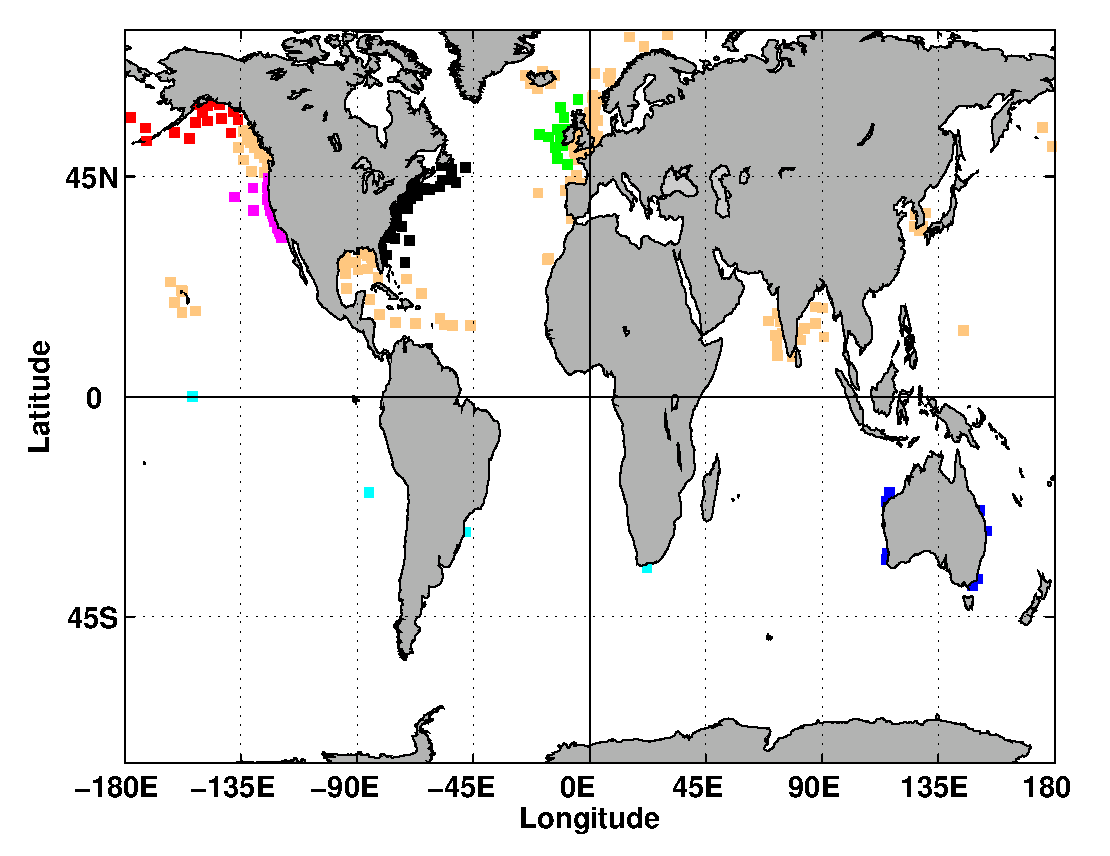
\includegraphics[width=12cm,height=8cm]{./figures/buoy_map.eps}
\caption{Location of buoys used in computing error metrics. Buoy data used in the present paper are color coded according to region and error metrics of each region are given in Fig.~\ref{fig:ecmwf_buoys_err}. ('Red' $ \rightarrow $ Alaska;'Magenta' $ \rightarrow $ US West Coast; 'Black' $ \rightarrow $ US East Coast; 'Green' $ \rightarrow $ Europe; 'Cyan' $ \rightarrow $ Southern Hemisphere; 'Blue' $ \rightarrow $ Australia)}
\label{fig:ecmwf_buoys}
\end{figure}

\setcounter{subfigure}{0}
\begin{figure}[t]
\subfigure[U.S. West Coast]{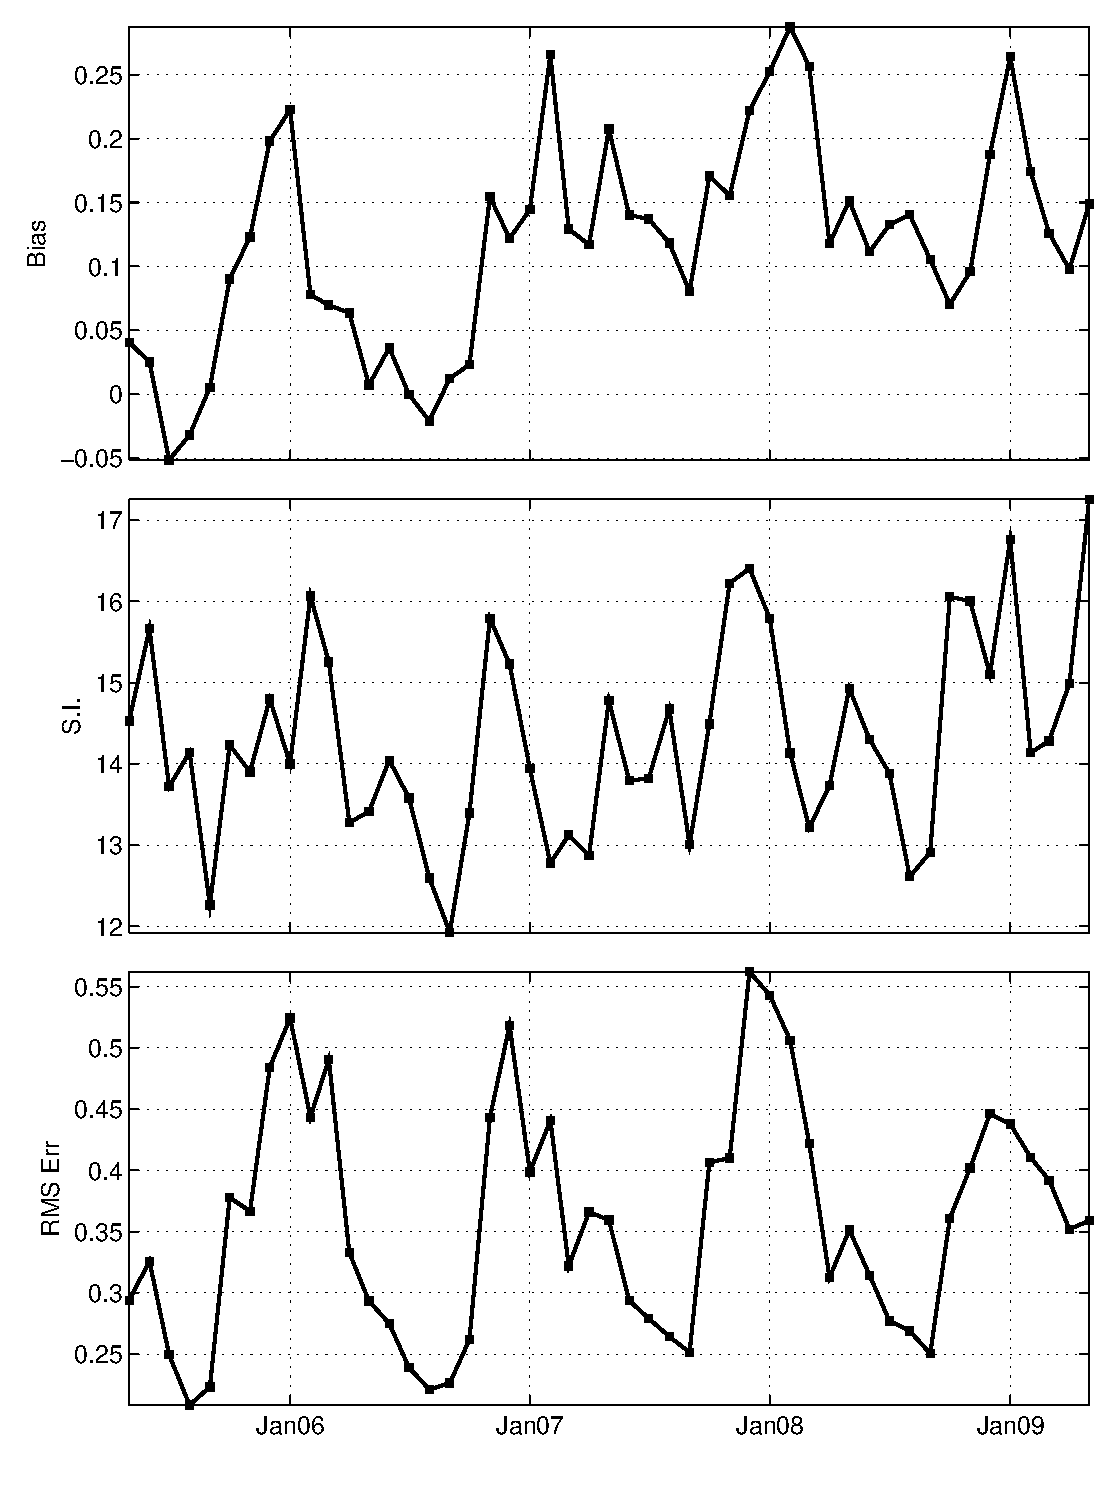
\includegraphics[width=5cm]{./figures/BulkStats2.Hs.US_West_Coast.eps}}
\subfigure[U.S. East Coast]{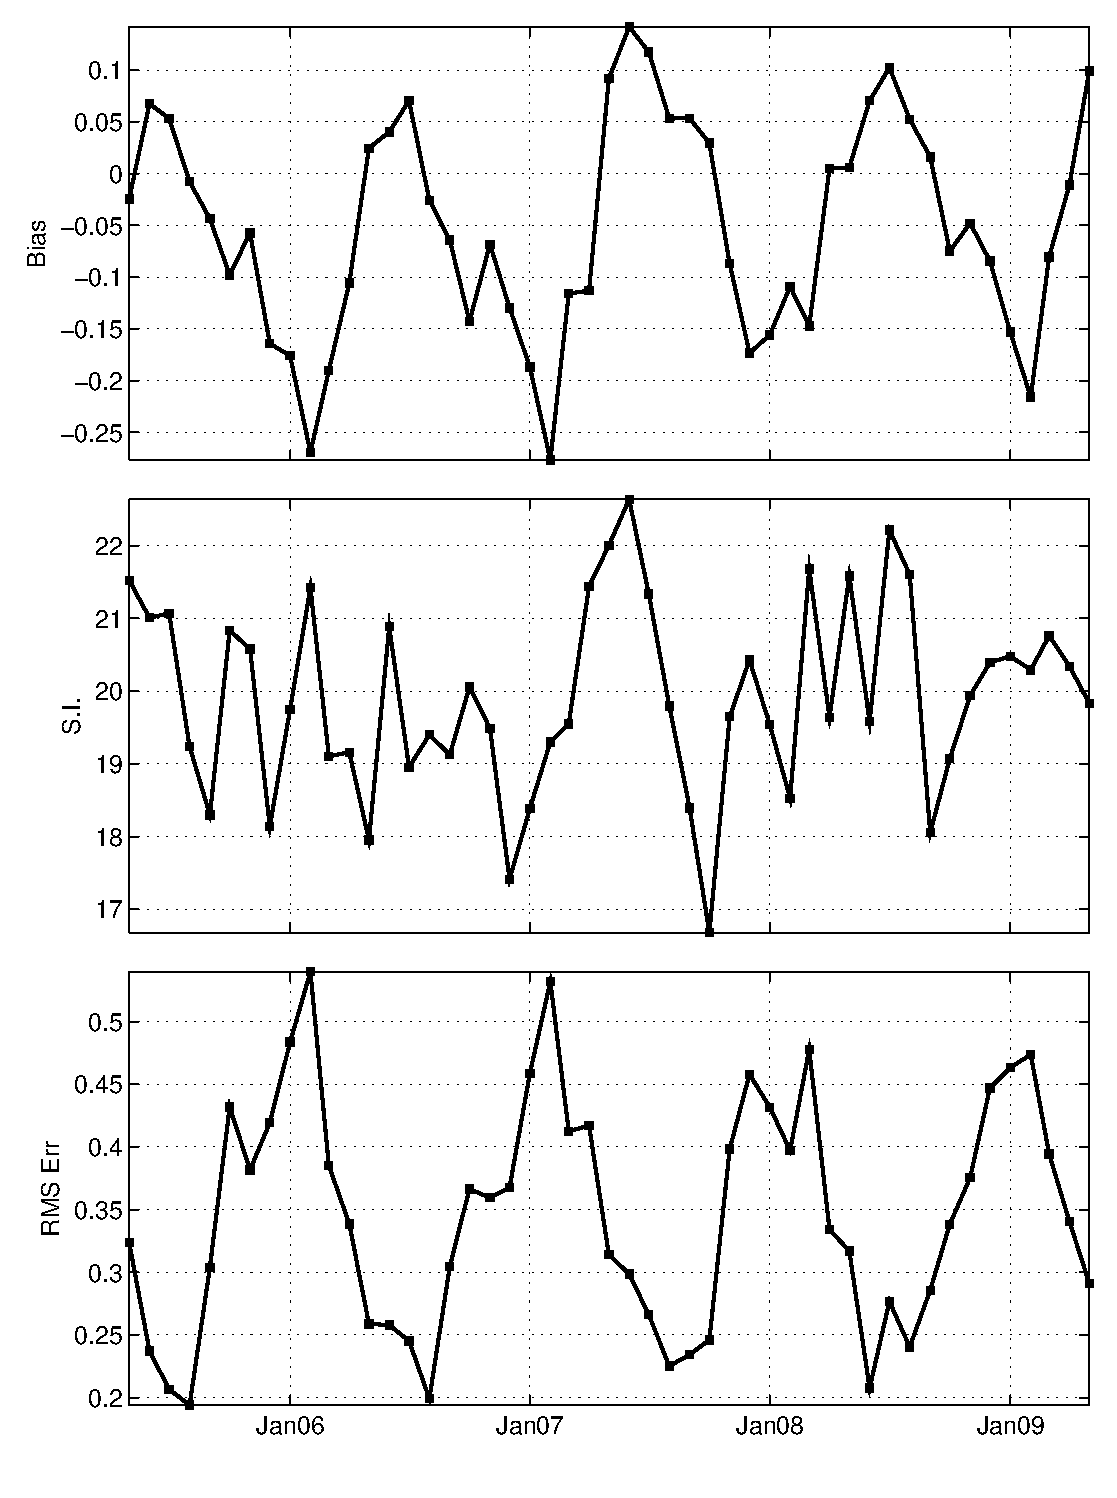
\includegraphics[width=5cm]{./figures/BulkStats2.Hs.US_eastcoast.eps}}
\subfigure[Alaska]{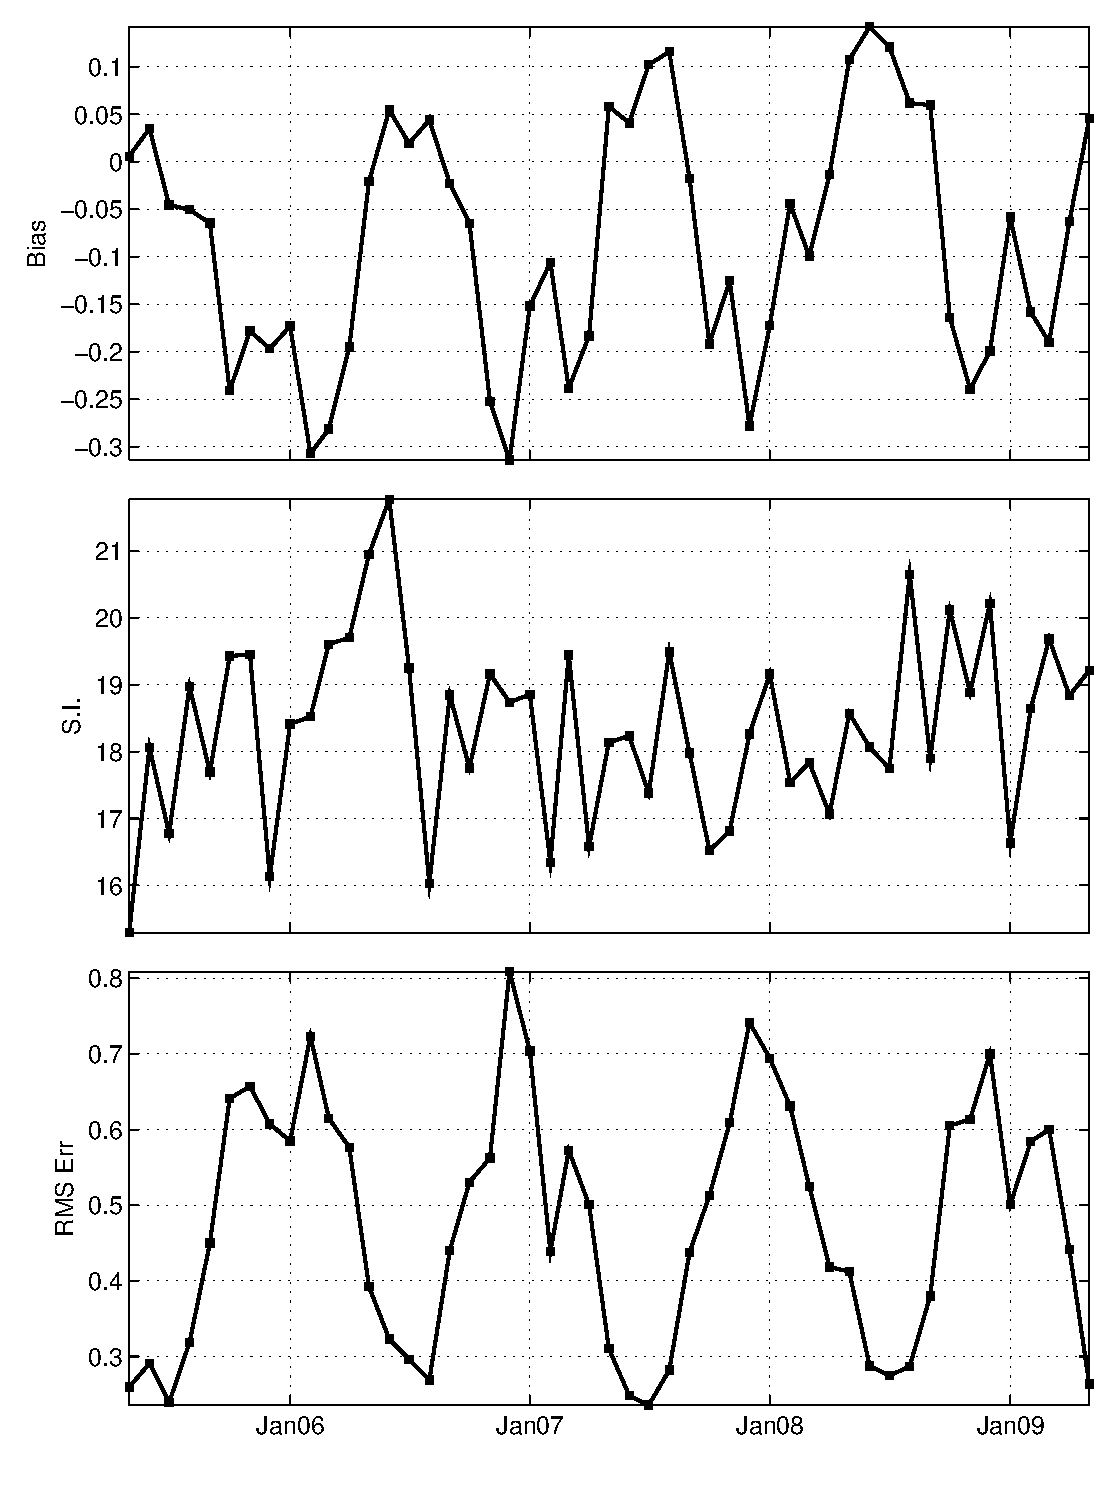
\includegraphics[width=5cm]{./figures/BulkStats2.Hs.Alaska.eps}}\\
\subfigure[Europe]{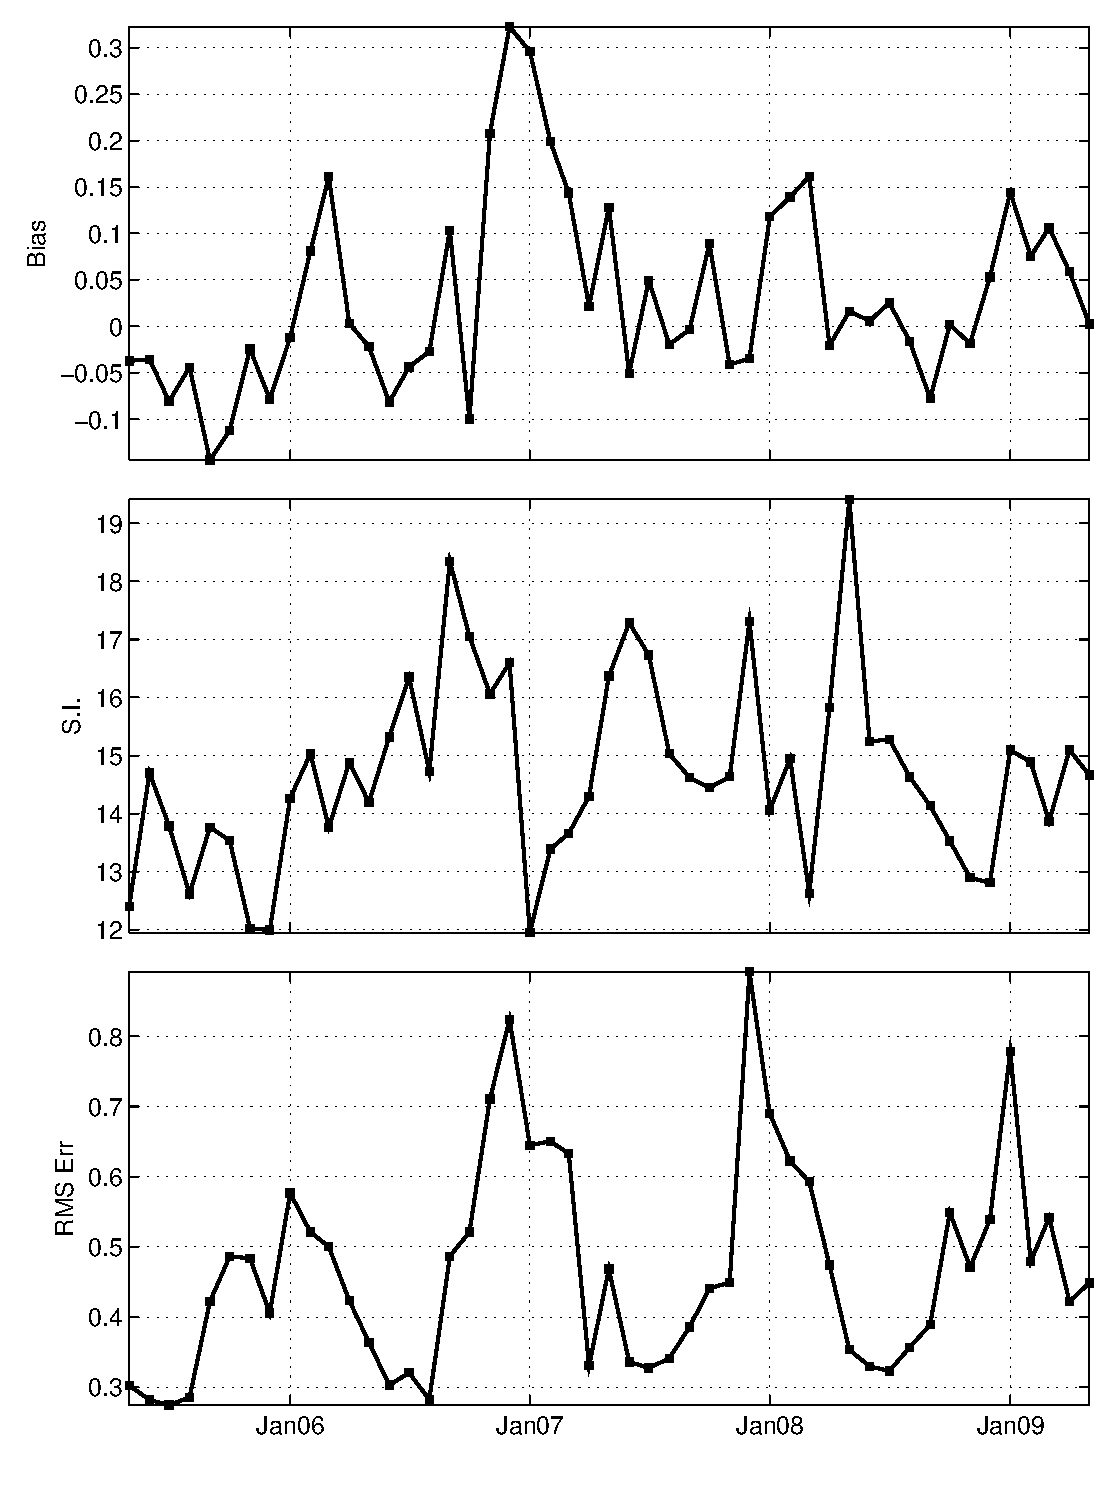
\includegraphics[width=5cm]{./figures/BulkStats2.Hs.Europe_Offshore.eps}}
\subfigure[Southern Hemisphere]{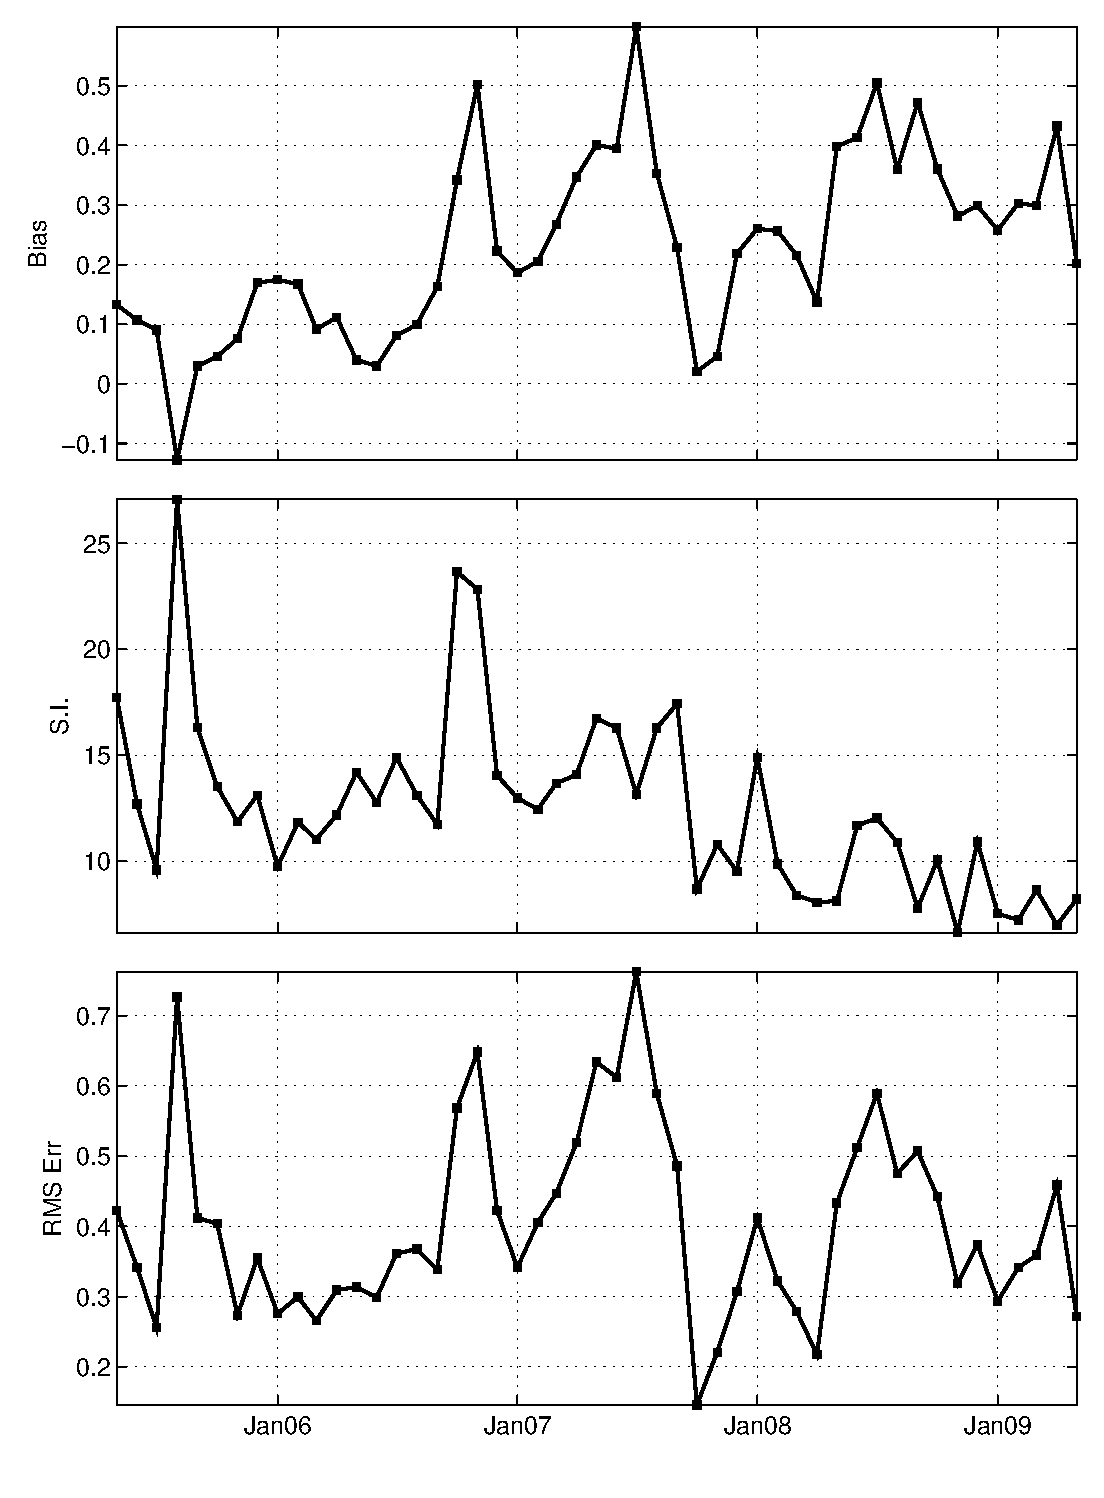
\includegraphics[width=5cm]{./figures/BulkStats2.Hs.Southern_Hemisphere.eps}}
\subfigure[Australia]{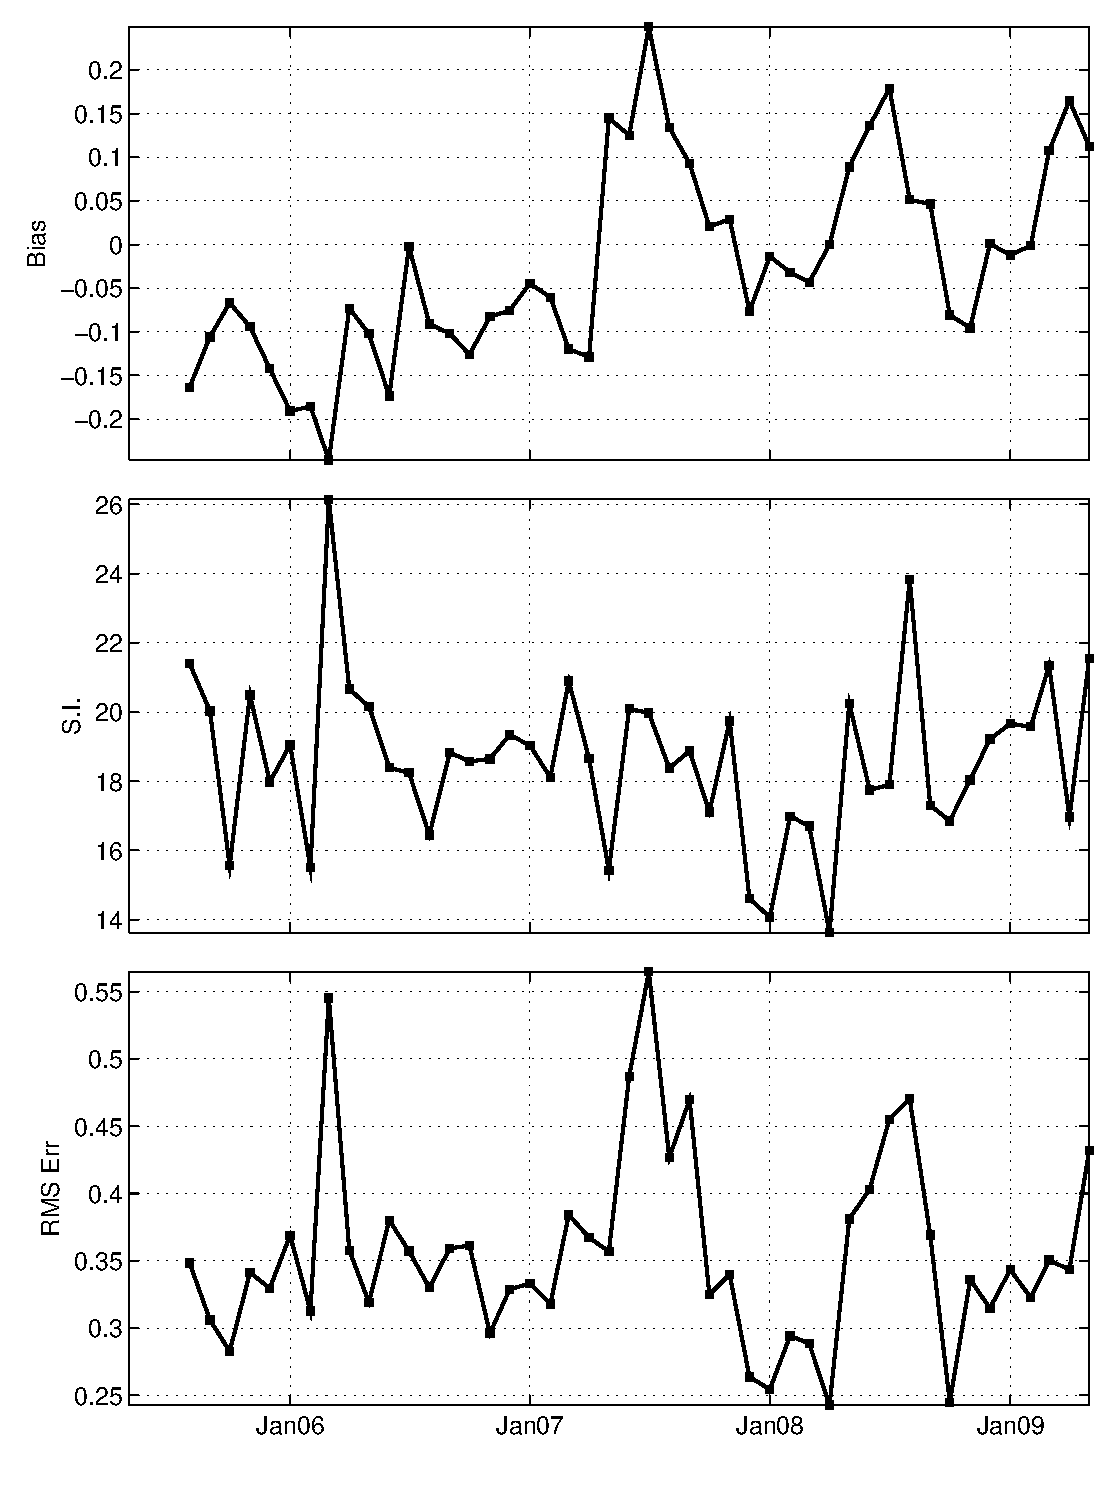
\includegraphics[width=5cm]{./figures/BulkStats2.Hs.Australia.eps}}
\caption{Error metrics of wave hindcast $Hs$ at buoys for the hindcast period of May 2005 through May 2009. Both bias and RMS error are in m. Map showing the buoy locations for each region is given in Fig~\ref{fig:ecmwf_buoys}.}
\label{fig:ecmwf_buoys_err}
\end{figure}

%\begin{figure}[t]
%  \noindent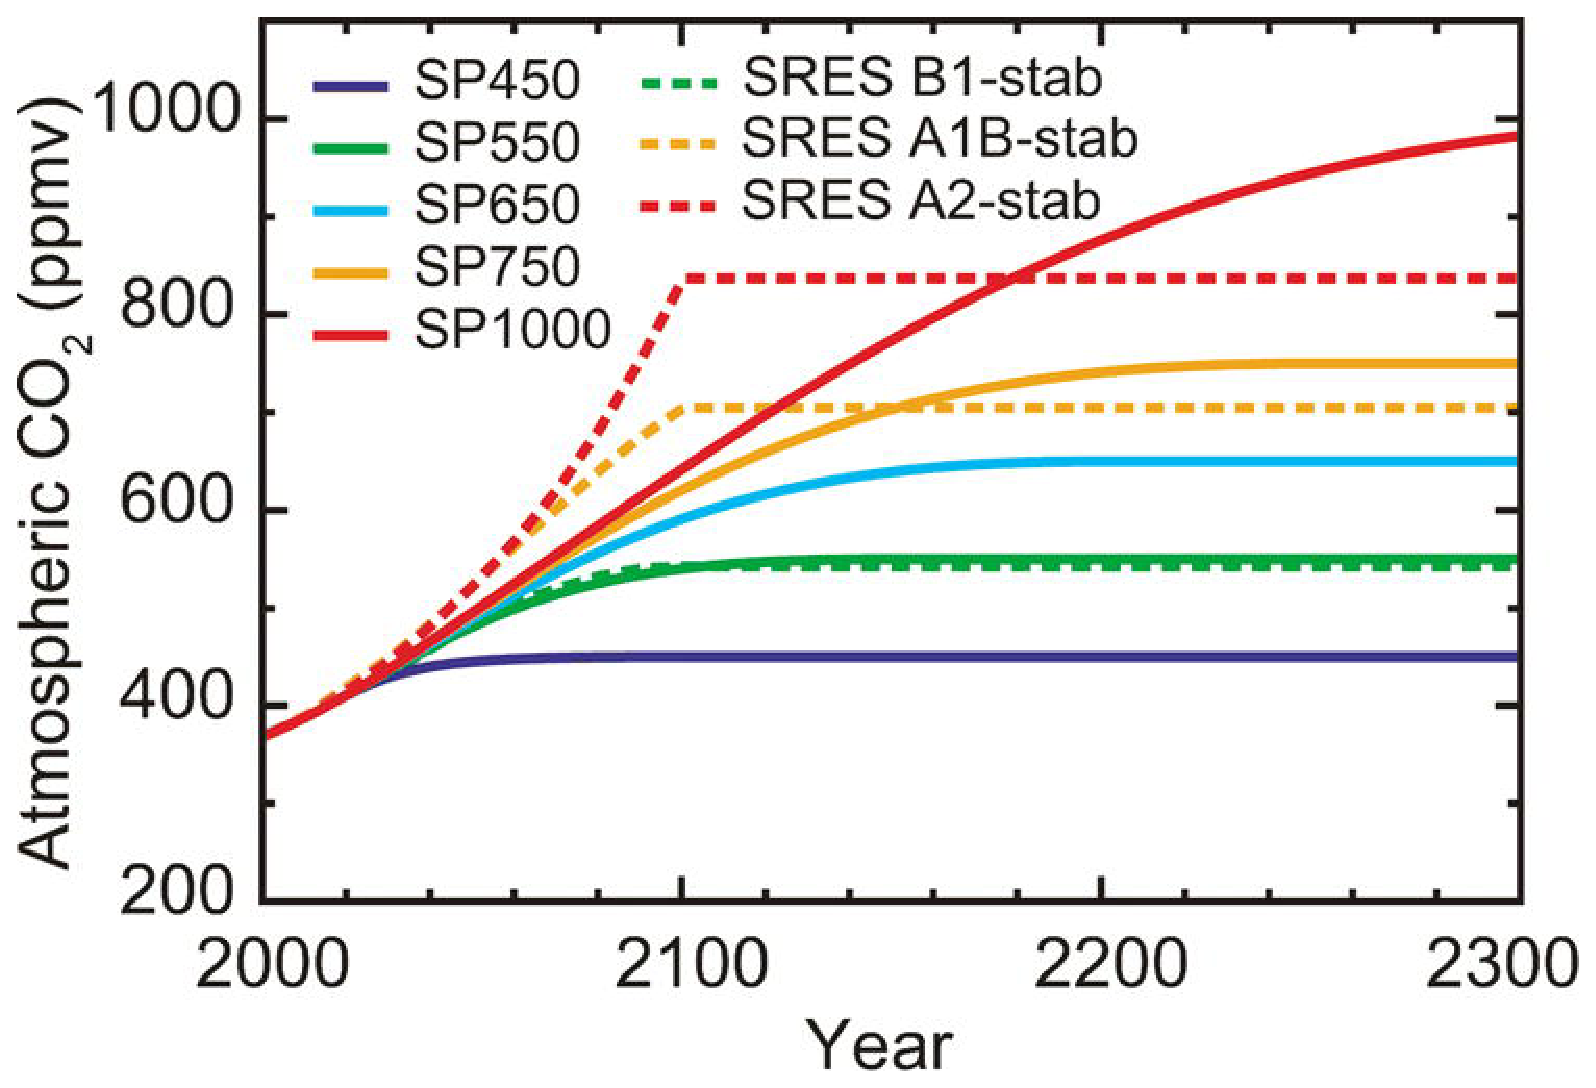
\includegraphics[width=19pc,angle=0]{./figures/figure01.eps}\\
%  \caption{Enter the caption for your figure here.  Repeat as
%  necessary for each of your figures. Create a figures directory and
%  place all figures in that directory. Figure from Houghton et al. (2001).}\label{f1}
%\end{figure}
%%%%%%%%%%%%%%%%%%%%%%%%%%%%%%%%%%%%%%%%%%%%%%%%%%%%%%%%%%%%%%%%%%%%%
% TABLES
%%%%%%%%%%%%%%%%%%%%%%%%%%%%%%%%%%%%%%%%%%%%%%%%%%%%%%%%%%%%%%%%%%%%%
%\begin{table}[t]
%\caption{This is a sample table caption and table layout.  Enter as many tables as
%  necessary at the end of your manuscript. Table from Lorenz (1963).}\label{t1}
%\begin{center}
%\begin{tabular}{ccccrrcrc}
%\hline\hline
%$N$ & $X$ & $Y$ & $Z$\\
%\hline
% 0000 & 0000 & 0010 & 0000 \\
% 0005 & 0004 & 0012 & 0000 \\
% 0010 & 0009 & 0020 & 0000 \\
% 0015 & 0016 & 0036 & 0002 \\
% 0020 & 0030 & 0066 & 0007 \\
% 0025 & 0054 & 0115 & 0024 \\
%\hline
%\end{tabular}
%\end{center}
%\end{table}
%
\end{document}